\documentclass[12pt,onecolumn,a4paper,final,notitlepage]{report}

\usepackage[left=3.5cm,top=2.5cm,right=2.5cm,bottom=2.5cm,includehead,includefoot]{geometry}

\usepackage{footnote}
%\makesavenoteenv{tabular} 

\usepackage[noend]{algorithmic}
\usepackage{algorithm}
\usepackage{todonotes}
\usepackage[MeX]{polski}
\usepackage{url}
\usepackage{graphicx}
\usepackage{float}
\usepackage[justification=centering]{caption}
%\usepackage{subfloat}
\usepackage{subfig}
\usepackage{amsmath}
\usepackage{amssymb}
%\usepackage[countmax]{subfloat}
\usepackage{wrapfig}

%\usepackage{listingsutf8}
%\usepackage[latin1]{inputenc}
% Euro characters etc.
%\usepackage{textcomp}
% Works perfectly with latin1
\usepackage{listings}

\lstloadlanguages{XML,C++}
\usepackage{color}
\linespread{1.3}
\definecolor{light-gray}{gray}{0.85}
\graphicspath{{./grafika/}}
% kodowanie: latin2, utf8 lub cp1250
\usepackage[utf8]{inputenc}
\floatname{algorithm}{Algorytm}
\numberwithin{algorithm}{chapter}
\usepackage{longtable}
\usepackage{multicol}
\newcommand{\sgn}{\text{sgn}}

\usepackage{fancyhdr}
\setlength{\headheight}{15pt}
\pagestyle{fancy}
\lhead{\fancyplain{}{\nouppercase\leftmark}}
\chead{}
\rhead{}
\lfoot{}
\cfoot{\fancyplain{}{\thepage}}
\rfoot{}

\definecolor{orange}{rgb}{1.0,0.3,0.2}


\begin{document}
\begin{titlepage}
\linespread{1.1}
\hspace{0.4cm}
 \begin{minipage}{0.4\textwidth}
	\begin{flushleft} 
	\includegraphics[scale=0.15]{./logo_pw_moje}
	\end{flushleft}
\end{minipage}
\begin{minipage}{0.4\textwidth}
	\begin{flushright} 
	\includegraphics[scale=0.6]{./logo_weiti}
	\end{flushright}
\end{minipage}
\begin{flushleft}


\end{flushleft}
\vspace{0.1cm}
\begin{center}
{\textbf{\LARGE POLITECHNIKA WARSZAWSKA}}\\
\Large Wydział Elektroniki i Technik Informacyjnych\\
\Large Instytut Systemów Elektronicznych\\[2.5cm]
 \begin{minipage}{0.9\textwidth}
	\begin{center} 
	\Large
	Maciej Gąbka\\nr albumu: 198404
	\end{center}
\end{minipage}
\\[1.5cm]
{\Large Praca dyplomowa magisterska}\\
 \Huge Sterowanie robotem - zawodnikiem rozgrywek RoboCup\\[2.0cm]
\begin{flushleft} \large
\hspace{5.5cm}Praca wykonana pod kierunkiem \\ 
\hspace{5.5cm}prof. dr hab. Jarosława Arabasa
\end{flushleft}
\vfill
% Bottom of the page
{\large Warszawa 2011}
\end{center}
\end{titlepage}

\input{./tex/streszczenie}

\tableofcontents

\chapter[Wstęp ]{Wstęp}
Szybki postęp technologiczny zapoczątkowany w XX wieku umożliwił rozwój nowych dziedziń nauki, między innymi robotyki. Obecnie maszyny mogą zastępować ludzi przy wykonywaniu wielu rozmaitych czynności.
Innowacyjne rozwiązania stwarzają jednak potrzebę opracowania wymagającego środowiska testowego. Jedną z takich inicjatyw, mających na celu wspieranie rozwoju i popularyzację robotyki są rozgrywki
RoboCup. W obrębie przedsięwzięcia wyróżnionych jest kilka lig, różniących się zasadami oraz typem robotów biorących udział w zawodach.
Głównym celem przyświecającym organizatorom jest stworzenie do 2050 roku drużyny robotów zdolnej wygrać z ówczesnymi mistrzami świata.
Liga RoboCup budzi zainteresowanie wielu ludzi na całym świecie, prace z nią związane  są prowadzone w wielu środowiskach akademickich na całym świecie.
W Polsce nie została jeszcze stworzona drużyna, która wystartowałaby w tych rozgrywkach.
Rozwiązanie problemu stawia przed uczestnikami wyzwania konstukcyjne oraz algorytmiczne. Niniejsza praca skupiona jest głównie na rowiązaniach algorytmicznych. Omówniony zostanie problem sterowania
zawodnikiem, wyznaczania bezkolizyjnej ścieżki do celu oraz reazlizacji prostych zachowań niezbędnych podczas rozgrywek.
\section{Zakres pracy}
Niniejsza praca jest niejako kontynuacją działań podjętych podczas realizacji pracy inżynierskiej. Tematyka w niej poruszona dotyczy na wstępie samych rozgrywek RoboCup. Jak już napisano we 
wstępie przedsięwzięcie dotyczny głównie rogrywek piłkarkich, w których udział biorą roboty. Jednak ze względu na dynamiczny rozwój samej robotyki do projektu dołączane są kolejne tematy.
Obecnie podział jest następujący:
\begin{itemize}
	\item \emph{RoboCupSoccer}, czyli rozgrywki piłkarskie autonomicznych robotów,
	\item \emph{RoboCupRescue}, obejmujący działania robotów w sytuacjach kryzysowych, czy niebezpiecznych dla ludzi,
	\item \emph{RoboCup@Home}, skupiający się na robotyce mającej na celu pomaganie człowiekowi w codziennych czynnościach,
	\item \emph{RoboCupJunior} popularyzujący robotykę wśród młodzieży.
\end{itemize}

Same rozgrywki piłkarskie \emph{RoboCupSoccer} także są podzielone na kilka lig, tutaj głównym kryterium jest konstrukcja mechaniczna zawodników. Więcej informacji na ten temat zostanie zaprezentowanych w rozdziale
\ref{chap:robocup}. W ramach samej pracy skupiono się na lidze małych robotów (\emph{Small-size League}), ponieważ już wcześniej prowadzone były prace w tym kierunku na Wydziale Elektroniki i 
Technik Informacyjnych Politechniki Warszawskiej.

W dalszej części pracy opisano nowe testowe środowisko symulacyjne oraz wprowadzone poprawki modyfikujące pracę symulatora.
Z racji, iż wczesniejsze prace prowadzono na symulatorze \emph{Player/Stage/Gazebo} zdecydowano się na dalsze prace na tej platformie.
Opracowane zostały nowe modele zawodników, wzorowane na rzeczywistych, holonomicznych
biorących udział w rozgrywkach. Opracowano sterownik (element symulatora) umożliwiający: kontrolę nad prędkością robota (wyposażono go dodatkowo w regulator PID), prowadzenie piłki jak i oddawanie strzału.
 W stosunku do poprzednich prac zdecydowano się także na implementację oraz poddanie testom nowego algorytmu nawigacji.  Rozwiązanie to zostało przetestowane w takich samych warunkach 
jak poprzednie. Dokonano także analizy i porównania otrzymanych wyników. Zaprezentowano także inne, stosowane w robotyce metody unikania kolizji. Jeden z nich także został zaimplementowany, w celu
rozwiązywania mniej złożonych zadań, takich jak odjechanie od przeszkody w momencie wystąpienia kolizji.

W pracy zostało przedstawione także jedno z podejść, powszechnie stosowane do koordynacji i planowania działań zawodników (\mbox{\texttt{STP - Skill Tactics Play}} \cite{stp}).
Zakłada ono planowanie zachowań drużyny na $3$ poziomach. Każdy odnosi się do innej warstwy abstrakcji.
\begin{enumerate} 
  \item Poziomem najwyżej w hierachii jest \texttt{Play}. Przez to pojęcie rozumiany jest plan gry dla całej drużyny, uwzględniana jest tutaj koordynacja
  poczynań pomiędzy zawodnikami. Plan zakłada przydział zawodnika do określonej roli. W oryginalnym rozwiązaniu role przydzielane są dynamicznie w zależności od sytuacji na boisku.
  W obrębie danego planu zawodnik wykonuje swoją rolę (sekwencję kilku \texttt{Tactics}), aż do momentu zakończenia danego planu lub wyznaczenia kolejnego.
  
  \item Przez \texttt{Tactics} rozumiany jest plan działań dla jednej roli. W taktyce zamknięte jest wykonywanie przez robota pojedynczej złożonej akcji.
  Przykładem może być strzał na bramkę. Robot dostaje polecenie oddania strzału na bramkę, zatem plan jego poczynań ma doprowadzić
 do sytuacji, w której osiągnie on pozycję umożliwiającą odddanie strzału na bramkę z zadanym powodzeniem.
 Plan na szczeblu pojedynczego robota jest wykonywany do momentu zmiany planu gry całej drużyny (ponownego przydziału robotów do ról).
 Przykładowe \texttt{Tactics}:
 \begin{itemize}
  \item strzał na bramkę,
  \item podanie piłki,
  \item odebranie podania,
  \item blokowanie innego robota,
  \item wyjście na pozycję,
  \item bronienie pozycji,
  \item dryblowanie z piłką.
 \end{itemize}
  Taktyka determinuje skończony automat stanów, w którym elementami są \texttt{Skills}. Wykonanie bieżącej taktyki sprwadza się do przechodzenia pomiędzy kolejnymi zachowaniami robota w obrębie
  danego automatu.
  \item Najniżej w hierarchii znajduje się pojęcie \texttt{Skills} odnosi się ono do konkretnych umiejętności robota, takich jak:
    \begin{itemize}
    \item przechwycenie piłki,
    \item oddanie strzału,
    \item doprowadzenie piłki do celu,
    \item przemieszczenie robota do celu,
    \item podążanie za innym robotem.
    \end{itemize}
  Na tym szczeblu nie wystąpuje koordynacja w obrębie drużyny. Zachowanie robota zmieniane jest w każdym kroku gry. Z każdego \texttt{Skill}, w każdym momencie określone musi być przejście
  albo do nowego zadania bądź kontynuowanie tego samego zadania. Przykładowo jeśli zlecimy robotowi przemieszczenie z piłką do celu i piłka 
  odskoczy robotowi, to powinien do niej podjechać, przechwycić ją, a następnie ponownie prowadzić do zadanego celu (należy jednak cały czas pamiętać, że jeśli nastąpi dobra okazja do strzału
na bramkę to należy z niej skorzysta.
\end{enumerate}

 W ramach pracy w pełni zrealizowane zostały dwie warstwy z oryginalnej hierarchii opisanej powyżej (\texttt{Skills} oraz \texttt{Tactics}). Aplikację projektowano w taki sposób, aby pozostawić miejsce
 na implementację warstwy \texttt{Play}, której niedkończono.
Użyteczność algorytmu sprawdzono podczas przeprowadzonych eksperymentów, wzorowanych na rzeczywistych zadaniach eliminacyjnych stosowanych w rozgrywkach RoboCup w ostatnich latach.

\section{Cel pracy}
Za główny cel niniejszej pracy postawiono przetestowanie użyteczności i skuteczności architektury \texttt{STP}. Aby jednak zrealizować to zadanie konieczne było
stworzenie środowiska symulacyjnego, umożliwiającego modelowanie rozgrywki \emph{Small-size League}. Przy opracowywaniu modelu środowiska starano się w jak największym stopniu odzwierciedlić realia
ligi \emph{Small-size League}. Po drugie środowisko symulacyjne miało być na tyle elastyczne, aby w przyszłości umożliwiało testowanie różnorodnych rozwiązań sterowania drużyną.
Zachowano schemat przepływu informacji z pracy inżynierskiej. Został on zamieszczony na rysunku \ref{fig:przeplyw_sterowania}. Stosowany w rozgrywach \emph{Small-size League} \texttt{videoserwer} został
zamodelowany jako osobna warstwa  aplikacji, komunikująca się bezpośrednio z symulatorem. Osobną warstwę stanowi także część aplikacji odpowiedzialna za sterowanie robotem.
\begin{figure}[H]
\centering
\includegraphics[scale=0.38]{./zalozenia/przeplyw_sterowania.pdf}
\caption{Komunikacja pomiędzy warstwami aplikacji.} \label{fig:przeplyw_sterowania}
\end{figure}
Główną motywacją takiej architektury było umożliwienie prostego przystosowania aplikacji do sterowania rzeczywistym robotem pobierającym dane z zewnętrznego serwera. 
Ponieważ w rozgrywkach biorą udział roboty holonomiczne, zdecydowano się na odejście od modelu robota o napędzie różnicowym stosowanego w pracy inżynierskiej (wzorowanego na \textit{HMT}) i opracowanie nowego wzorowanego na rzeczywistych
zawodnikach.
Kolejnym celem pracy wynikającym bezpośrednio ze zmiany modelu zawodnika, było zaimplementowanie i przetestowanie algorytmu nawigacji robota w dynamicznym środowisku. Zdecydowano się na algorytm \texttt{RRT},
postanowiono także porównać jego skuteczność z wcześniej stosowanym \texttt{CVM}.



\chapter{Liga Robocup \label{chap:robocup}}
\section{Opis projektu Robocup \label{sec:opis_robocup}}
	Projekt Robocup, jego idea jak i historia zostały opisane w pracy inżynierskiej \cite{inzynierka}, więcej informacji na temat mistrzost można także znaleźć na oficjalnej stronie projektu
	\mbox{\url{http://www.robocup.org}}. W niniejszej pracy problematyka rozgrywek robotów w piłkę nożną zostanie przedstawiona jedynie skrótowo ze szczególnym uwzględnieniem
	budowy robota wykorzystywanego w lidze na której wzorowano się podczas prac.
	Głównym celem przedsięwzięcia jest stworzenie do 2050 roku drużyny w pełni autonomicznych robotów humanoidalnych zdolnych wygrać rozgrywkę z aktualnymi mistrzami 
	świata.
	Aby osiągnąć zamierzony cel należy połączyć osiągnięcia z różnych dziedzin nauki. Przede wszystkim ważna jest konstrukcja zarówno mechaniczna jak i elektroniczna
	robota. Zawodnik powinien być wyposażony w odpowiedni zestaw czujników umożliwiających osiągnięcie pełnej autonomiczności. 
	Z drugiej strony natomiast należy dysponować funkcjonalnym oprogramowaniem umożliwiającym współpracę wielu robotów.
	Projekt jest realizowany nieprzerwanie od września 1993 roku. Początkowo brali w nim udział jedynie przedstawiciele środowisk naukowych z Japonii.
	Rozgrywki toczone są w kilku niezależnych od siebie ligach.
	Aktualnie wyróżnione zostały nastepujące ligi:
	\begin{itemize}
	\item liga symulacyjna
	\item \emph{Small-size League}
	\item \emph{Middle-size League}
	\item \emph{Standard Platform League }
	\item \emph{Humanoid League}
	\end{itemize}
	Liga symulacyjna jest pewnego rodzaju grą, w której uczestniczące drużyny implentują program decydujący o zachowaniu zawodników.
	Jest ona najstarszą z lig, towarzyszy przedsięwzięciu od samego początku jego istnienia.
	Zachowanie robotów jest symulowane za pomocą programu zwanego \emph{Robocup Soccer Simulator}.

	Kolejną z lig jest \emph{Small-Size League}. W rozgrywkach tej ligi drużyna składa się maksymalnie z pięciu niewielkich robotów, takich jak widoczne na fotografii \ref{fig:F180}. 
	Roboty  nie są jednak w pełni autonomiczne, ponieważ nie
	posiadają własnych sensorów. Algorytm sterujący czerpie informację o~położeniu piłki oraz robotów z kamery
	umieszczonej centralnie nad boiskiem. Lidze tej został poświęcony w całości paragraf \ref{sec:F180}.	
	\begin{figure}[ht]
	\centering
	\includegraphics[scale=0.7]{./liga_robocup/F180}
	\caption{ Roboty biorące udział w \emph{Small-Size League}\newline(źródło: \texttt{www.robocup.org})} \label{fig:F180}
	\end{figure}
	
	\emph{Middle-size League} to rozgrywki w pełni autonomicznych robotów. W odróżnieniu od wcześniej omawianej
	ligi małych robotów, globalny system wizyjny jest całkowicie zakazany. Każdy robot jest wyposażony w osobny zestaw czujników wizyjnych.
	Zadaniem zawodników jest reagowanie na sytuację na planszy i koordynowanie swoich działań w zależności od zachowań innych graczy.

	W projekcie wyróżnione są także ligi \emph{Standard Platform League }, czyli rozgrywki piesków \textit{Aibo} konstruowanych przez firmę \textit{Sony} oraz 
	liga robotów humanoidalnych. W tej ostatniej biorę udział roboty przypominające swoją budową ludzi czyli posiadać korpus, nogi, ręce oraz głowę.
	\section{Szczegółowe omówienie ligi Small-size (F180)}
	\subsection{Zasady}
	Zbiór zasad obowiązujący w lidze podlega co roku aktualizacji przez komitet techniczny ligi. Zazwyczaj około
	rok przed kolejnymi mistrzostwami znane są zasady na nich obowiązujące. Początkowo w rozgrywkach wszystkie
	roboty  korzystały  z globalnego systemu wizyjnego, jednak w  trakcie kolejnych zmian w przepisach
	dopuszczono do rozgrywek roboty z własnym systemem wizyjnym, dzięki czemu  zaczęto wykorzystywać także
	rozproszone algorytmy sterowania.
	
	W rozgrywce na boisku o wymiarach 7.4~[m] na 5.4~[m] wyłożonej zielonym dywanem lub wykładziną biorą udział dwie
	drużyny składające się z maksymalnie pięciu robotów. Jeden z robotów może zostać oddelegowany do pełnienia
	funkcji bramkarza, jednak powinno to zostać zgłoszone przed rozpoczęciem meczu. 
	Konstrukcja robota powinna zmieścić się w walcu o średnicy 18~[cm] oraz wysokości 15~[cm]. W przypadku robotów z
	własnymi sensorami wizyjnymi dopuszcza się wysokość do 22.5~[cm]. Robot może być wyposażony w urządzenie do prowadzenia piłki, jednak istnieją pewne ograniczenia dotyczące
	jego budowy oraz stosowania w czasie gry. Mianowicie robot może prowadzić piłkę maksymalnie przez dystans
	50~[cm], po przejechaniu którego powinien albo podać ją innemu zawodnikowi, albo kopnąć przed siebie i dalej ją
	prowadzić. W przeciwnym wypadku sygnalizowane jest przewinienie. Natomiast konstrukcja urządzenia do dryblowania nie może uniemożliwiać kontaktu z piłką zawodnikowi z przeciwnej drużyny.
		
	Rozgrywka jest całkowicie kontrolowana przez arbitra, który czuwa nad tym, aby  regulamin był przestrzegany. Do
	jego zadań należy sygnalizowanie przewinień, zdobytych bramek oraz innych typowych sytuacji na boisku.
	Sędzia ma prawo zmienić swoją decyzje po konsultacjach z asystentem. Postanowienia arbitra są tłumaczone na
	sygnały elektryczne przez asystenta i wysyłane do wszystkich zawodników.

	\subsection{Schemat komunikacji}
	Jedną z najistotniejszych spraw podczas rozgrywki jest dostęp do informacji o położeniu piłki
	i pozostałych robotów. Aby rozwiązać ten problem drużyny uczestniczące w rozgrywce mogą korzystać z systemu wizyjnego widocznego na rysunku~\ref{fig:comunication}. 
	Składa się on z kamery ustawionej centralnie nad boiskiem oraz specjalnej aplikacji \mbox{\emph{RoboCup VideoServer}}\footnote{ Do pobrania z \url{http://sourceforge.net/projects/robocup-video}}. 
	Obraz zarejestrowany przez kamerę jest przesyłany do komputera, na którym uruchomiony jest \emph{RoboCup VideoServer}. Program przetwarza na bieżąco obraz z kamery i w wyniku swojego działania dostarcza informację 
	o położeniu oraz prędkościach robotów i piłki. Dane te następnie są wykorzystywane przez rywalizujące ze sobą drużyny na potrzeby ich algorytmów sterujących zawodnikami.
 	Algorytm sterujący jako wynik swojego działania powinien zwracać kierunek i prędkość zawodników. Ta ostateczna informacja jest wysyłana droga radiową do zawodnika.
	Sam program \mbox{\emph{RoboCup VideoServer}} oferuje bardzo dużą funkcjonalność. Pozwala przykładowo dokonać dokładnej
	kalibracji nawet w przypadku, gdy boisko widziane przez kamerę ma kształt owalny (z powodu zniekształceń obrazu). Przed rozpoczęciem pracy z aplikacją
	należy zdefiniować początek układu współrzędnych oraz rozpoznawane przez serwer kolory.
	\begin{figure}[H]
	\centering
	\includegraphics[ scale=0.5]{./liga_robocup/dataflow}
	\caption{Schemat komunikacji w  \mbox{\emph{Small Size League}}\newline(źródło: \texttt{www.robocup.org}) }
	\label{fig:comunication}
	\end{figure} 	
	\mbox{\emph{RoboCup VideoServer}} może rozpoznawać nie tylko położenie poszczególnych robotów, ale także ich orientację na
	płaszczyźnie. Jednak do tego celu niezbędne jest zastosowanie specjalnych znaczników. Każdej z drużyn przed rozpoczęciem rozgrywki zostaje przypisana para kolorów, jakie zawiera znacznik. Dzięki zastosowaniu dwóch kolorów możliwe jest nie tylko rozróżniania robotów z różnych drużyn, ale także właśnie ich orientacji.

\section{Budowa robota \label{sec:budowa_robota} w \emph{Small-size League}}
	W oficjalnym regulaminie ligi nie zostały narzucone konkretne modele robotów, które mogą brać udział w
	rozgrywkach, jednak, obserwując kolejne mistrzostwa, łatwo zauważyć, że wśród zgłaszanych drużyn dominuje jedna konstrukcja mechaniczna. Została ona zaprezentowana na  rysunkach \ref{fig:F180_budowa}.
 	\begin{figure}
	\centering
	\subfloat[]{\label{fig:F180_budowa1}\includegraphics[ scale=0.34]{./liga_robocup/F180_budowa1}}
	\subfloat[]{\label{fig:F180_budowa2}\includegraphics[ scale=0.38]{./liga_robocup/F180_budowa2}}
	\subfloat[]{\label{fig:F180_budowa3}\includegraphics[ scale=0.38]{./liga_robocup/F180_budowa3}}
	\caption{Popularny model robota wykorzystywany w \mbox{lidze \emph{F180}}\newline(źródło: \texttt{www.robocup.org}) }
	\label{fig:F180_budowa}
	\end{figure}
	Podczas gry w piłkę nożną często wynika potrzeba zmiany orientacji w miejscu. W prezentowanym rozwiązaniu
	zdecydowano się na omnikierunkową bazę jezdną. Składa się ona z trzech kół szwedzkich, w tym dwóch niezależnie
	napędzanych. Koło szwedzkie posiada taką zaletę, iż dodatkowo poza obrotem wokół własnej osi umożliwia obrót
	wokół punktu styczności koła z podłożem oraz wokół osi rolek umieszczonych na kole.
	\begin{wrapfigure}{r}{0.42\textwidth}
	\vspace{-30pt}
	\begin{center}	
	\includegraphics[width=0.38\textwidth]{./liga_robocup/znacznik}
	\end{center}
	\vspace{-10pt}	
	\caption{Znacznik umożliwiający systemowi wizyjnemu identyfikację robotów \label{fig:znacznik}}
	\vspace{-10pt}
	\end{wrapfigure}
	Dzięki zastosowaniu takiego rozwiązania uzyskano w pełni holonomiczną budową robota.
	Robot biorący udział w rozgrywkach musi być zdolny do prowadzenia piłki. Zastosowana konstrukcja jest wyposażona w urządzenie do dryblowania widoczne na rysunkach \ref{fig:F180_budowa1} oraz \ref{fig:F180_budowa3}. 
	Zbudowane jest ono z walca nadającego piłce wsteczną rotację, przez co nie odbija się ona od robota, a także nie traci on nad nią kontroli w momencie hamowania lub obracania się.
	W regulaminie rozgrywek dopuszczono do stosowania jedynie urządzenia do dryblowania 
	działające na piłkę siłą
	prostopadłą do podłoża rys.~\ref{fig:F180_budowa1} (we wcześniejszych latach w użyciu były  urządzenia, w których obracany walec był umieszczony pionowo).

	Ostatnim ważnym elementem, w który musi być wyposażony robot, jest znacznik (rys.~\ref{fig:znacznik}).
	Znajduje się on w takim miejscu, aby kamera umieszczona centralnie nad boiskiem mogła go zarejestrować (przykrywa robota od góry).
	Znaczniki umożliwiają systemowi wizyjnemu określenie, do której drużyny należy dany robot, a także poprawne rozpoznanie jego pozycji, orientacji oraz prędkości
	na boisku.



\chapter[Player/Stage/Gazebo ]{Player/Stage/Gazebo \label{chap:gazebo}}
\chaptermark{Player/Stage/Gazebo}
	Symulator \mbox{\texttt{Player/Stage/Gazebo}} został już opisany w pracy inżynierskiej \cite{inzynierka} jednak z uwagi na jego ważną rolę i zmiany jakie zdecydowano się wprowadzić w symulowanym
	środowkisku podczas rozwijania aplikiacji zdecydowano się na krótkie przypomnienie koncepcji projektu.

	\section{Koncepcja}
	Początki oprogramowania nazwanego \textit{Project Player} (oznaczającego zestaw trzech aplikacji: \textit{Player}, \textit{Stage} oraz \textit{Gazebo}) 
	sięgają 1998 roku, kiedy to
 	na Uniwersytecie Południowej Kaliforni w Los Angeles rozpoczęto prace nad stworzeniem oprogramowania pozwalającego 
 	na sterowanie grupą robotów mobilnych \textit{Pioneer~2} firmy ActivMedia, będących na wyposażeniu tamtejszego laboratorium robotyki. 
	Twórcami projektu byli Brian Gerkey i Richard Vaughan, później dołaczyli do nich Kasper St{\o}y oraz Andrew Howard.
	Do tego czasu w skład stworzonego oprogramowania wchodziły: \textit{Golem} (pozwalający na sterowanie
	robotem \textit{Pioneer}) oraz \textit{Arena} (symulator). W toku prac narodziła się idea opracowania uniwersalnego zestawu aplikacji, umożliwiającego kontrolę nad robotami niezależnie od zastosowanych rozwiązań sprzętowych, 
	dobrze współpracującego z symulatorem oraz dostępnego za darmo (zgodnie z GNU GPL). 
	Tak powstały aplikacje \textit{Player} oraz \textit{Stage}. \textit{Player} miał za zadanie dostarczać narzędzi do sterowania podzespołami robota, 
	a \textit{Stage} stanowił prosty dwuwymiarowy symulator. Oprogramowanie to znalazło szeroko stosowane 
	zarówno w uczelnianych laboratoriach, jak i wśród indywidualnych użytkowników. W 2002 roku rozpoczęto prace
	nad nowym symulatorem \textit{Gazebo}, który miał służyć do modelowania zachowań robotów w trójwymiarowym świecie 
	z uwzględnieniem rzeczywistych oddziaływań fizycznych między obiektami. Całość projektu jest w dalszym ciągu intensywnie rozwijana przez
	deweloperów oraz aktywną społeczność użytkowników. Oprogramowanie działa na systemach Linux, Solaris, *BSD oraz Mac OSX. 
	Szczegółowe informacje, dokumentacja oraz kody źródłowe każdej z aplikacji dostępne są pod adresem \url{http://playerstage.sourceforge.net/}.
	W trakcie prac nad opisywaną aplikacją wydana została stabilna wersja symulatora i zmieniona strona internetowa projektu, obecnie jest on dostępny pod \url{http://gazebosim.org/}.
	
	\section{Architektura symulatora}
	\begin{figure}[!b]
	\centering
	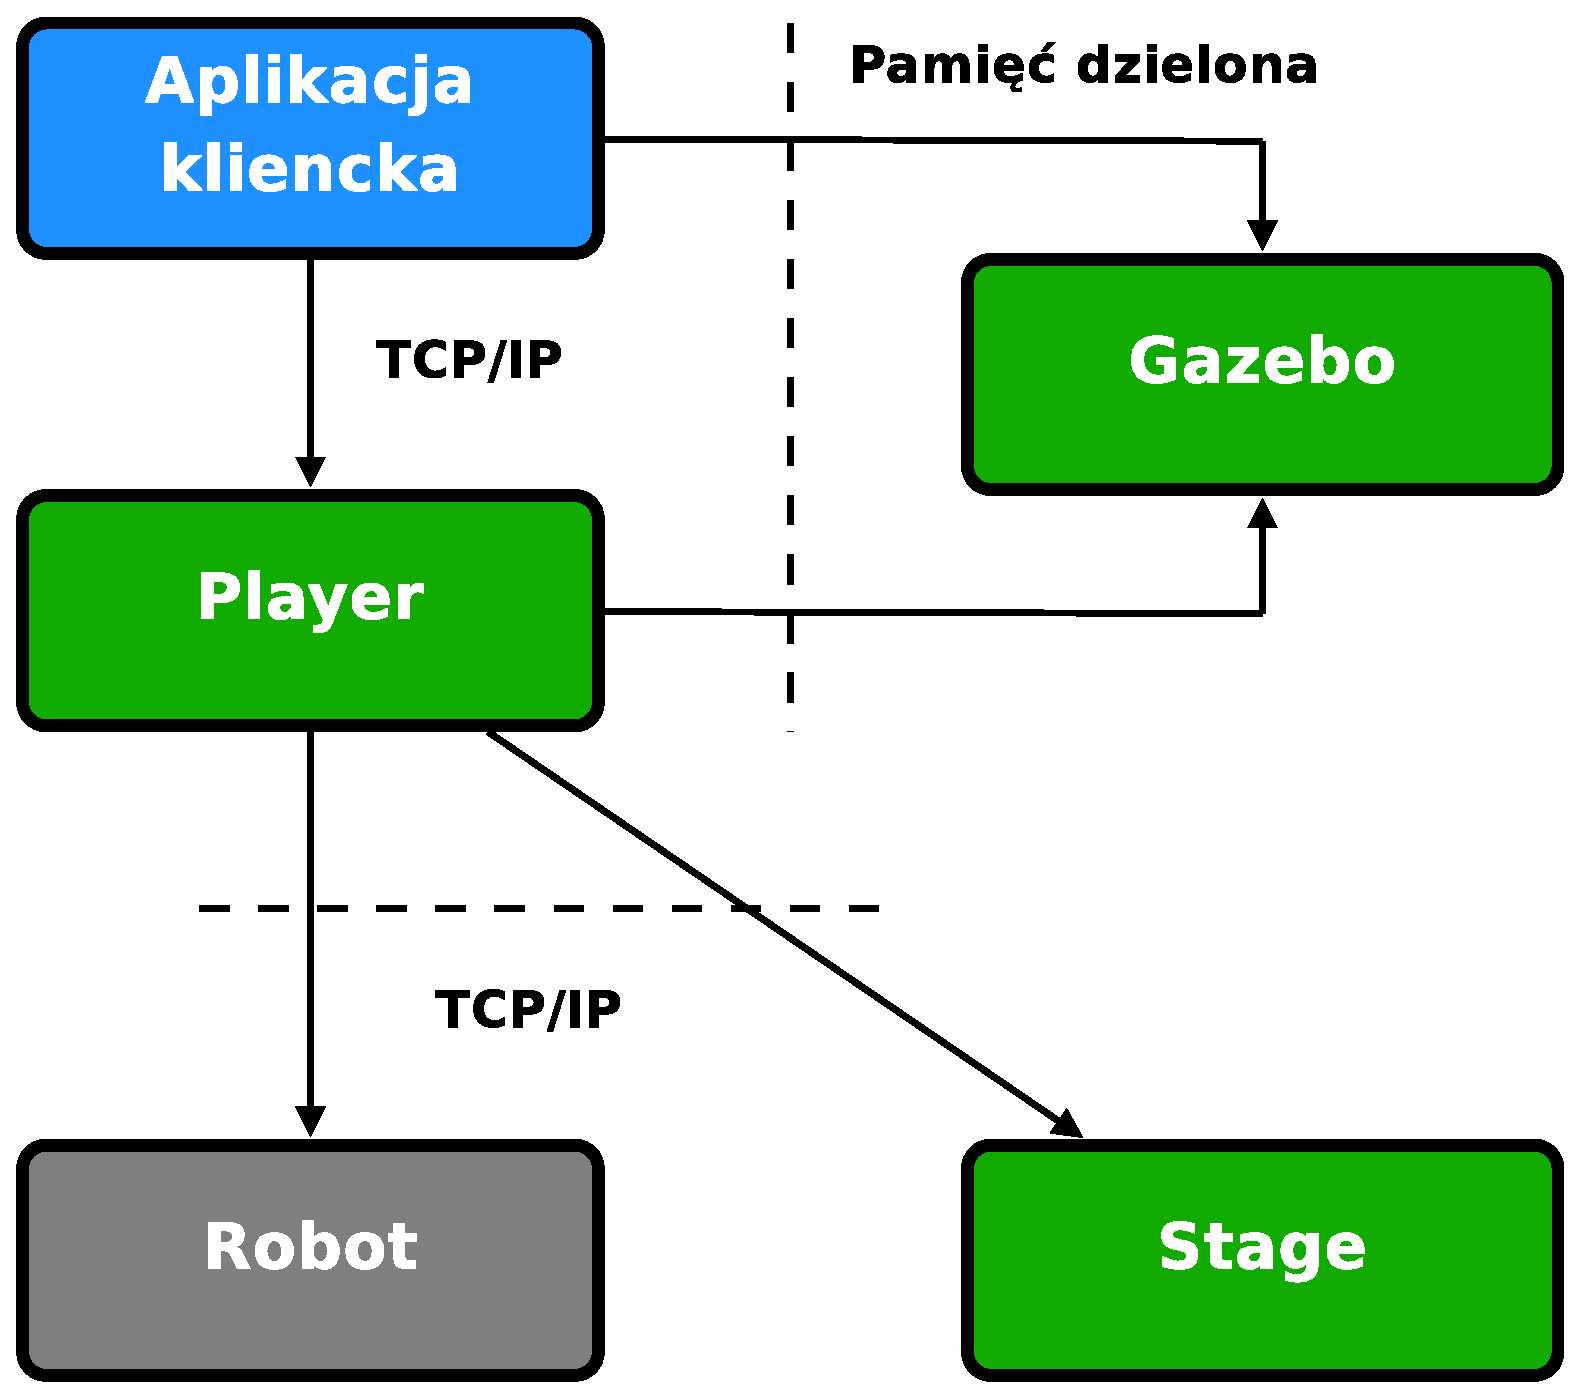
\includegraphics[scale=0.3]{./gazebo/architektura}
	\caption{Schemat komunikacji w środowisku \textit{Player/Stage/Gazebo} \label{fig:arch}}
	\end{figure}
	
	Schemat zależności pomiędzy komponentami \textit{Player/Stage/Gazebo} został przedstawiony na 
	rysunku~\ref{fig:arch}.
	Dobrze obrazuje on rolę programu \textit{Player}, pełniącego funkcję pośrednika pomiędzy aplikacją klienta 
	(odpowiadającą za algorytm sterowania robotem) a rzeczywistym robotem lub symulatorami modelującymi jego zachowanie (\textit{Stage} oraz \textit{Gazebo}). Do komunikacji 
	pomiędzy komponentami wykorzystywany jest protokół TCP/IP. Aplikacja kliencka łączy się z ``serwerem'', którego
	rolę pełni \textit{Player}. Z punktu widzenia klienta nie ma znaczenia, czy interfejsy dostarczane przez \textit{Playera} sterują robotem rzeczywistym,
	czy tylko jego wirtualnym odpowiednikiem (modelem) w jednym z symulatorów. Ponadto, przeniesienie kontroli
	pomiędzy symulowanym a rzeczywistym robotem wymaga tylko nieznacznych modyfikacji kodu.

	Istnieje jeszcze druga opcja -- do każdego z symulatorów (\textit{Stage} lub \textit{Gazebo}) można odwoływać się bezpośrednio w przypadku,
	gdy korzystanie z \textit{Playera} nie jest uzasadnione, lub gdy chce się dokonać pewnych modyfikacji w sposobie
	działania symulatora. Do tego celu zostały stworzone biblioteki (\textit{libstage} oraz \textit{libgazebo}), 
	które dostarczają funkcji służących do komunikacji między aplikacją kliencką, a symulatorami.
	\begin{figure}[h]
	\centering
	\includegraphics[scale=0.3]{./gazebo/wybrana_architektura}
	\caption{Zrealizowany schemat komunikacji w środowisku \textit{Player/Stage/Gazebo} \label{fig:wybrana_arch}}
	\end{figure}
	Podsumowując, struktura pakietu oprogramowania \mbox{\textit{Player/Stage/Gazebo}} umożliwia tworzenie aplikacji sterujących robotami w sposób, który zapewnia przenośność stworzonych programów i ich działanie zarówno na symulatorach robotów, jaki i na rzeczywistych obiektach.
	
 	\subsection{Gazebo}
 	
 	Program \textit{Gazebo}, podobnie jak \textit{Stage}, umożliwia symulację grup robotów mobilnych. Różnica polega na tym, że symulowane
 	środowisko jest trójwymiarowe, uwzględnia dynamikę, cechy fizyczne oraz oddziaływania między modelami. Wiąże się
 	to oczywiście ze wzrostem potrzebnej mocy obliczeniowej, dlatego też symulowane grupy robotów nie
 	mogą być tak liczne, jak w przypadku \textit{Stage}.
 	 	
 	\textit{Gazebo} zostało oparte na nastepujących komponentach:
 	\begin{itemize}
 	 \item ODE\footnote{Open Dynamics Engine, \url{http://www.ode.org}}, bibliotece  odpowiadającej za symulację
 	 	cech fizycznych brył oraz detekcję kolizji,
 	 \item OGRE\footnote{Object-Oriented Graphics Rendering Engine, \url{http://www.ogre3d.org/}}, 
		silniku graficznym umożliwiającym tworzenie wspomaganej sprzętowo grafiki 3D,
 	 \item FLTK\footnote{Fast Light Toolkit, \url{http://www.fltk.org/}}, bibliotece dostarczającej 
		przenośny interfejs użytkownika dla Gazebo,
	 \item libXML2\footnote{ \url{http://xmlsoft.org/}}, parserze XML (stworzonym oryginalnie dla środowiska graficznego GNOME), umożliwiającym Gazebo proste wczytywanie plików konfiguracyjnych.
 	\end{itemize}

	\textit{Gazebo} pozwala na symulację standardowych sensorów (m.in. czujniki odległości, kamery, GPS). Dostarcza gotowe modele 
	popularnych robotów (jak np. \textit{Pioneer2DX}, \textit{Pioneer 2AT} oraz \textit{SegwayRMP}). Pozwala ponadto na tworzenie własnych modeli
	i definiowanie ich własności fizycznych (takich jak np. masa, współczynnik tarcia, sztywność), co zapewnia odpowiedni realizm
	symulacji i pozwala na interakcję z innymi obiektami (podnoszenie, przesuwanie brył itp.). Co więcej, dla każdego z modeli
	dostępne są kontrolery pozwalające na ich sterowanie, ale nic nie stoi na przeszkodzie, żeby zdefiniować własne według potrzeb i dodać je do \textit{Gazebo}. 
	\begin{figure}[!t]
	\centering
	\label{fig:gazebo}
	\includegraphics[scale=0.42]{./gazebo/gazebo_screen}
	\caption{\textit{Gazebo} -- okno główne (wersja 0.10)}
	\end{figure}

 	\subsection{Player}
 	
 	\textit{Player} jest serwerem sieciowym dostarczającym interfejs do kontroli nad sensorami i efektorami, w które wyposażony jest robot,
	za pośrednictwem protokołu TCP/IP. Jak już wspomniano, został zaprojektowany do obsługi robotów z rodziny \textit{Pioneer 2} firmy ActivMedia, jednak z czasem rozbudowano go dodając obsługę wielu innych urządzeń i algorytmów\footnote{Aktualną listę można znaleźć pod adresem \url{http://playerstage.sourceforge.net/doc/Player-cvs/player/supported_hardware.html}}. Najważniejsze cechy decydujące o atrakcyjności i funkcjonalności Playera to:
	\begin{itemize}
	 \item niezależność od platformy i stosowanego języka programowania -- program klienta łączący się z aplikacją \textit{Playera} może zostać uruchomiony na dowolnym systemie operacyjnym; wymagane jest tylko istnienie połączenia sieciowego z robotem oraz to, żeby język programowania, w którym napisano progam kliencki, potrafił obsługiwać komunikację za pośrednictwem socketów TCP; \textit{Player} dostarcza obecnie narzędzia ułatwiające komunikację z nim w językach C, C++, Tcl, Java, Python i Common LISP,
	 \item brak ograniczeń na strukturę programu klienta przeznaczonego do sterowania robotem -- może ona być wielowątkowa, napisana w prosty sposób reaktywny (pobierz dane - reaguj) lub bardziej skomplikowany -- z perspektywy \textit{Playera} nie ma to żadnego znaczenia,
	 \item możliwość reprezentacji wielu urządzeń przez ten sam interfejs -- dzięki temu można np. sterować dwoma zupełnie różnymi robotami za pomocą tego samego programu klienta (ich efektory odpowiadające za przemieszczanie robota będą w obu przypadkach reprezentowane przez interfejs \textit{position}),
	 \item wspieranie dowolnej liczby klientów; przykładowo, można stworzyć wiele połączeń do dowolnych instancji aplikacji \textit{Playera} na dowolnym robocie i za pomocą jednej aplikacji sterować robotami, podczas gdy druga będzie odpowiedzialna za generowanie wykresów obrazujących odczyty z sensorów,
	 \item możliwość zdalnej konfiguracji serwera w czasie jego pracy,
	 \item łatwość testowania rozwiązań w symulatorach -- \textit{Player} jest kompatybilny ze Stage oraz Gazebo, a kod napisany w celu sterowania robotami może działać bez poprawek zarówno z symulatorem, jak i z rzeczywistym robotem.
	\end{itemize}

	\section{Modelowanie obiektów w Gazebo}
	Filozofia modelowania w \textit{Gazebo} opiera się na tworzeniu opisu świata (o parametrach określonych 
	w pliku \textit{.world} za pomocą języka XML), w którym umieszczone zostają symulowane obiekty. Plik zawiera informacje o dodanych do świata modelach, ale także parametry określające przebieg symulacji, takie 
	jak krok pracy symulatora czy sposób detekcji kolizji. 
	\subsection{Zasady modelowania w Gazebo 0.10}
	Opis modelowanego świata powinien zawierać się w pliku głównym z rozszerzeniem \textit{.world}.
	W pliku muszą być zapisane informacje związane z konfiguracją interfejsu użytkownika, sposobem renderowania sceny oraz fizyką symulacji.
	Elementy przykładowego pliku \textit{.world} zostały zaprezentowane na listingach poniżej.
	%\small
	%\lstset{language=XML,  basicstyle=\ttfamily\footnotesize,
	\lstset{language=XML,  basicstyle=\ttfamily\scriptsize, 
	commentstyle={}, xleftmargin=20pt, numbers=left, numberstyle=\footnotesize,
	caption={},
	backgroundcolor=\color{light-gray},
	frame=single,
	breaklines=true}
	\begin{lstlisting}[name=gazebo_simple_world]
	<?xml version="1.0"?>
	<gazebo:world>
	\end{lstlisting}
	Bardzo istotnym elementem jest konfiguracja fizyki (ODE), interfejs umożliwia konfigurację globalnych parametrów takich jak:
	\begin{lstlisting}[name=gazebo_simple_world]
	<physics:ode>
		<stepTime>0.001</stepTime>
		<gravity>0 0 -9.8</gravity>		
		<erp>0.8</erp>
		<cfm>0.05</cfm>
		<stepType>quick</stepType>
		<stepIters>25</stepIters>
		<stepW>1.4</stepW>
		<contactSurfaceLayer>0.007</contactSurfaceLayer>
		<contactMaxCorrectingVel>100</contactMaxCorrectingVel>
	 </physics:ode>
	\end{lstlisting}
	\lstset{language=XML,  basicstyle=\ttfamily\footnotesize, 
	commentstyle={}, xleftmargin=20pt, numbers=left, numberstyle=\footnotesize,
	caption={},
	backgroundcolor=\color{light-gray},
	frame=single,
	breaklines=true}
	Znaczenie poszczególnych parametrów jest następujące:
	\begin {enumerate}
	 \item \texttt{stepTime} jest wyrażony w sekundach i określa czas pomiędzy kolejnymi aktualizacjami silnika \texttt{ODE},
	 \item \texttt{gravity} jest wektorem określającym siłę grawitacji,
	 \item \texttt{erp} rozwija się na \textit{error reduction parameter}, przyjmuje on wartości z przedziału od $0$ do $1$ i jest odpowiedzialny za redukcję błędów w połączeniach pomiędzy bryłami
	  (problematyka zostanie szerzej poruszona na stronie \pageref{fig:joints}); \texttt{erp} ustawione na $0$ powoduje, że żadna dodatkowa siła nie jest przykładana do danej bryły, natomiast wartość $1$
	 powoduje, że wszytskie błędy połączeń zostaną naprawione w kolejnym kroku symulatora,
	 \item \texttt{cfm} jest skrótem od \textit{constraint force mixing} i odpowiada za sztywność ograniczeń występujacych w kolizjach między bryłami, gdy wartość jest równa $0$ ograniczenie wynikające z fizyki
nie może zostać złamane, ustawienie parametru na wartość dodatnią powoduje, że ograniczenie staje się ``miękkie'', sprężyste,
	  
	 \item \texttt{stepType} odpowiada za rodzaj używanej funkcji z \texttt{ODE} do detekcji kolizji, użytkownik może dokonać wybrou jednej z dwóch wartości:
	      \begin{itemize}
	       \item \textit{world}, używana jest wtedy funkcja \texttt{dWorldStep}, operująca na macierzy zawierającej wszystkie ograniczenia, złożoność obliczeniowa tej metody wynosi $m^3$, natomiast pamięciowa
jest rzędu $m^2$, gdzie $m$ określa ilość wierszy (ograniczeń) analizowanej macierzy,
	       \item \textit{quick}, do detekcji kolizji stosowana jest metoda iteracyjna, w literaturze nazywana \texttt{SOR - Successive over-relaxation} należąca do rodziny metod Gaussa–Seidela, jej złożoność obliczeniowa jest rzędu $m*N$,
		a pamięciowa $m$, gdzie $m$ ma znaczenie jak wyżej,
		natomiast $N$ jest liczbą iteracji; dla dużych systemów metoda jest dużo bardziej wydajna jednak mniej dokładna, mogą także występować problemy z jej stabilnością; najprostszą metodą na poprawę stabilności
		jest zwiększanie \texttt{cfm}, 
	      \end{itemize}
	 \item \texttt{stepIters} - ilość iteracji, gdy do detekcji kolizji wybrano metodę \textit{quick},
	 \item \texttt{stepW} określa czas relaksacji metody Gaussa–Seidela, 
	 \item \texttt{contactSurfaceLayer} określa głębokość na jaką może wnikać bryła w podłoże, ustawienie parametru na małą wartość dodatnią zapobiega jitterowi w momencie, gdy ograniczenia są nieustannie tworzone
	  i zrywane (na przykład podczas ruchu koła po podłożu),
	 \item \texttt{contactMaxCorrectingVel} jest maksymalną korektą prędkości jaka może wynikać z utworzonych tymczasowo kontaktów; domyślnie parametr przyjmuje nieskończoną wartość.
	  \todo{przetlumaczyc na polski}Reducing this value can help prevent "popping" of deeply embedded objects. 
	\end {enumerate}
	Warto wspomnieć, że niektóre parametry można zmieniać dla poszczególnych modeli lub połączeń \textit{joints}.\newline
	Ustawienia interfejsu: typ (dostępne tylko \textit{fltk}), rozmiaru okna i jego pozycja początkowej:
\begin{lstlisting} [name=gazebo_simple_world]
    <rendering:gui>
        <type>fltk</type>
        <size>640 480</size>
        <pos>0 0</pos>
    </rendering:gui>
\end{lstlisting}
	Określenie parametrów renderowanej sceny: techniki cieniowania, tekstury pokrywającej niebo (dostępne inne opcje, jak np. rodzaje oświetlenia, dodawanie mgły itp.):
\begin{lstlisting} [name=gazebo_simple_world]
    <rendering:ogre>
        <shadowTechnique>stencilAdditive</shadowTechnique>
        <sky>
              <material>Gazebo/CloudySky</material>
        </sky>
    </rendering:ogre>
</gazebo:world>
\end{lstlisting}

	Do tak stworzonego pliku z opisem świata należy następnie dodać modele.  Dodany obiekt musi zawierać co najmniej jeden element \textit{body}, który jest złożony z elementów \textit{geoms}. Sekcja opisująca przykładowy model piłki mogłaby wyglądać następująco:
	\begin{figure}[H]
	\centering
	\includegraphics[scale=0.35]{./gazebo/geoms}
	\caption[Dostępne typy \textit{geoms}]
		{\label{fig:geoms}Dostępne typy \textit{geoms} -- Gazebo 0.10 (źródło:~\cite{gazebo_experts})}
	\end{figure}
	
	\lstset{language=XML,  basicstyle=\ttfamily\footnotesize, 
	commentstyle={}, xleftmargin=20pt, numbers=left, numberstyle=\footnotesize,
	caption={},
	backgroundcolor=\color{light-gray},
	frame=single,
	breaklines=true}
\begin{lstlisting}[name=gazebo_przyklad_pilka]
<model:physical name="ball">
    <static>false</static>
\end{lstlisting}
Na wstępie deklarowany jest model, którego parametr \textit{static} ustawiono na \textit{false}, co oznacza, że będzie on brał udział
w symulacji fizycznej i może oddziaływać z innymi obiektami. Następnie należy zadeklarować ``ciało'' tworzonego obiektu:
\begin{lstlisting}[name=gazebo_przyklad_pilka]
    <body:sphere name = "ball_body">	
\end{lstlisting}
Wewnątrz \textit{body}, które jest odpowiedzialne za dynamikę obiektu, należy umieścić elementy opisujące kształt obiektu (pozwalające tym samym na detekcję kolizji) -- w tym przypadku zdefiniowano kulę o wymiarach i masie odpowiadającej piłce do golfa:
\begin{lstlisting}[name=gazebo_przyklad_pilka]
	<geom:sphere name = "ball_geom">
		<xyz>0 0 0.01</xyz>
		<rpy>0 0 0 </rpy>
		<size>0.02</size>
		<mass>0.045</mass>
\end{lstlisting}
Sekcja \textit{visual} bloku \textit{geom} pozwala na przypisanie obiektowi wyglądu -- może to być figura o dowolnym kształcie (stworzona np. w programie do grafiki 3D) i wybranej przez projektanta teksturze lub kolorze:
\begin{lstlisting}[name=gazebo_przyklad_pilka]
		<visual>	
			<scale>0.02 0.02 0.02</scale>
			<size>0.02</size>
			<mesh>unit_sphere</mesh>
			<material>Gazebo/Orange</material>
		</visual>
	</geom:sphere>				
    </body:sphere>
</model:physical>
\end{lstlisting}	


	
	\subsubsection{Połączenia pomiędzy bryłami }
	Tworząc modele, można korzystać z trzech podstawowych brył (kula, walec, prostopadłościan), a także z siatek \textit{trimesh} oraz elementów \textit{height field} (stworzonych do generowana terenu -- por. rys. \ref{fig:geoms})).
	Żeby zamodelować robota, należy jeszcze stworzone bryły odpowiednio ze sobą powiązać. Do tego służą elementy typu \textit{joint}, którymi można łączyć komponenty \textit{body} (modelujące np. koła i podwozie robota).
	Stopnie swobody połączenia zależą od wybranego typu wiązania \textit{joint} (dostępne typy przedstawiono na rys. \ref{fig:joints}). Obiekty połączone wiązaniem tworzą parę kinematyczną.
	\textit{Gazebo} umożliwia nadawanie tak połączonym bryłom prędkości obrotowych względem siebie, co pozwala na modelowanie ruchomych elementów robotów.
	\begin{figure}[H]
	\centering
	\includegraphics[scale=0.43]{./gazebo/joints}
	\caption{Typy połączeń \textit{joints} (Źródło: dokumentacja ODE) \label{fig:joints}}
	\end{figure}
	Jak wspomniano wcześniej, w czasie realizowanej symulacji połączenia pomiędzy bryłami moga ulec wypaczeniu, na skutek sił działających na model. Może to być tarcie,
	siła powodująca obrót bryły czy siły działające na model podczas kolizji. Sytacje taką przedstawiono na rysunku \ref{fig:bad_joint}.
	\begin{figure}[H]
	\centering
	\includegraphics[scale=0.43]{./gazebo/bad_joint}
	\caption{Zepsute połączenie (\textit{joints}) (Źródło: dokumentacja ODE) \label{fig:bad_joint}}
	\end{figure}
	Błędy tego typu można redukować za pomocą parametru \texttt{erp} ustawianego globalnie lub dla każdego z połączeń indywidualnie.
	\subsubsection{Sterowniki modeli }
	Sterowanie zaprojektowanym modelem jest możliwe po uprzednim wyposażeniu go w sterownik (\textit{controller}). Sterowniki implentowane są przez użytkownika w $C++$ jako klasa dziedzicząca
	po zdefiniowanym w \textit{libgazebo} interfejsie. Klasa odpowiada za przetwarzanie danych z sensorów robota oraz pozwala
	na zadawanie prędkości bryłom połączonym wiązaniami. Komunikuje się on z programem sterującym za pośrednictwem interfejsów (bezpośrednio korzystając z \textit{libgazebo} lub poprzez \textit{Playera}).
	\textit{Gazebo} oczywiście dostarcza gotowe sterowniki, pozwalające na kontrolowanie np. robota z napędem różnicowym, w wersji $0.10$ dodano także przykładowy model robota holonomicznego zawarty
	w pliku \textit{wizbot.world}. Aby z nich skorzystać, wystarczy przypisać wybrany sterownik do modelu robota, określić, które ze złączeń odpowiadają jego kołom i podać nazwę instancji interfejsu,
	za pomocą którego odbywać ma się komunikacja pomiędzy klientem a sterownikiem. W przypadku sterowania przemieszczeniem będzie to interfejs \textit{position}, za pomocą którego możemy zadawać prędkości bryłom,
	ale \textit{Gazebo} posiada też zaimplementowane interfejsy do sterowania innymi elementami np. do komunikacji z laserowymi czujnikami odległości, kamerą bądź chwytakiem manipulatora. 
	\lstset{language=XML,  basicstyle=\ttfamily\footnotesize, 
	commentstyle={}, xleftmargin=20pt, numbers=left, numberstyle=\footnotesize,
	caption={Przykład przypisanie sterownika do modelu},
	backgroundcolor=\color{light-gray},
	frame=single,
	breaklines=true}
	\begin{lstlisting}
<model:physical name="pioneer_model">
    <controller:pioneer2dx_position2d name="controller">
        <leftJoint>left_hinge_joint</leftJoint>
        <rightJoint>right_hinge_joint</rightJoint>
        <interface:position name="position_iface"/>
    </controller>
</model:physical>
	\end{lstlisting}	

	
	\subsection{Realizacja środowiska Ligi RoboCup \label{subsect:realizacjaROBOCUP} }
	
	W celu realizacji niniejszej pracy stworzono dla symulatora \textit{Gazebo} modele odpowiadające robotom biorącym udział w \emph{Small-size League}. 
	Boisko zostało stworzone z wykorzystaniem rzeczywistych wymiarów($5.4[m] x 7.4[m]$). 
	Zgodnie z regułami Ligi z 2007 roku\protect\footnote{\url{http://small-size.informatik.uni-bremen.de/rules/f180rules2007.html}} utworzono również linie boiska, 
	pozostawiając wystarczającą dla robota przestrzeń przy bandach tak, żeby było możliwe np. wykonywanie zagrań z autu. 
	Model piłki odpowiada piłce do golfa, której używa się w oficjalnych rozgrywkach.
	
	\begin{figure}[!b]
	\centering
	\includegraphics[scale=0.4]{./gazebo/roboty}
	\caption{Opracowane modele robotów (oparte na konstrukcji HMT)}
	\end{figure}

	Wykonane modele robotów wzorowano na konstrukcji rzeczywistych robotów wykorzystywanych w \emph{Small-size League}.
	Główna częścią robota jest walec o promieniu $6[cm]$ i wysokości $4[cm]$, umieszczony na trzech kołach rozmieszczonych symetrycznie na podstawie walca.
	Robot został dodatkowo wyposażony w \textit{dribbler}\protect\footnote{urządzenie opisano w par.~\ref{sec:budowa_robota}} pomagający utrzymać kontrolę nad piłką.
	Mimo że \textit{Gazebo} udostepnia sterownik dla napędu holonomicznego, sterowanie robotem wymagało napisania nowego kontrolera, ponieważ nie uwzględniał on obsługi
	\textit{dribblera}. Kod źródłowy sterownika został zamieszczony na płycie CD razem z kodem źródłowym wykorzystywanej wersji symulatora.	
	\begin{figure}[H]
	\centering
	\includegraphics[scale=0.4]{./gazebo/boisko.png}
	\caption{Model boiska}
	\end{figure}

	W trakcie prac nad modelowaniem Ligi wprowadzono kilka poprawek w symulatorze. Aby zamodelować w pełni koło szwedzkie należało dodać możliwośc określenia
	w jakim kierunku dla danej bryły występuje tarcie. W tym celu w skecji opisującej bryłę dodano nowy parametr:
	\lstset{language=XML,  basicstyle=\ttfamily\footnotesize, 
	commentstyle={}, xleftmargin=20pt, numbers=left, numberstyle=\footnotesize,
	caption={Parametr określający kierunek siły tarcia},
	backgroundcolor=\color{light-gray},
	frame=single,
	breaklines=true}
	\begin{lstlisting}	
	<fDir1>1 0 0</fDir1>
	\end{lstlisting}
	Powyższa wartość oznacza, że tarcie występuje jedynie w kierunku osi $OX$ danej bryły.
	\todo{opisac jak zaimplentowano w ode brak tarcia}

\chapter[Sterowanie modelem robota z \emph{Small-size League}]{Sterowanie modelem robota z \emph{Small-size League} \label{chap:holonomic}}
%\chaptermark{holonomic}
Budowę i napęd robota należy dobrać odpowiednio do postawionego zadania. W przypadku ligi \emph{Small-size League}, najważniejszym elementem jest prostota i mobilność
takiej jednostki, w pracy inżynierskiej \cite{inzynierka} posługiwano się robotem modelem robota o napędzie różnicowym (dwa niezależnie napędzane koła). Decyzję o odwzorowaniu takiego robota
w symulatorze motywowano wtedy próbą odzwierciedlenia rzeczywistego robota \texttt{HMT} \cite{hamada_mgr} stworzonego w ramach koła robotyki \texttt{Bionik} działającego na Wydziale Elektroniki i Technik Informacyjnych Politechniki
Warszawskiej. W niniejszej pracy zrezygnowano jednak z tego modelu, ponieważ nie był wystarczająco funkcjonalny. Zdecydowano się natomiast na zbudowanie modelu wzorowanego na rzeczywistym zawodniku \emph{Small-size League}.  
\section{Omówienie omnikierunkowej bazy jezdnej}
Analogicznie jak podczas rzeczywistej rozgrywki, decydującym elementem jest budowa anatomiczna i zdolności motoryczne zawodników, tak samo podczas
rozgrywek robotów istotna rolę odgrywa baza jezdna zawodników. W pracy inżynierskiej testom poddawany był robot o napędzie różnicowym. Baza ta posiadała jednak 
znaczące ograniczenia, które musiały zostać uwzględnione w algorytmach sterujących. Praktyczniejszą w użyciu jest baza omnikierunkowa. Korzystając z takiej bazy w
większości algorytmów robot może być traktowany jako punkt materialny.
\subsection{Opis położenia kół}
Baza omnikierunkowa składa się z umieszczonych symetrycznie co najmniej trzech kół szwedzkich tak jak zaprezentowano to na rysunku \ref{fig:holonomic_base}.
Każde z kół posiada osobny napęd. Budowę koła omnikierunkowego przedstawiono na ilustracji \ref{fig:omnidirectional_wheel}. 
\begin{figure}[h]
\centering
\includegraphics[scale=0.7]{./holonomic/holonomic_base}
\caption{ Rozkład kół w omnikierunkowej bazie jezdnej }\label{fig:holonomic_base}
\end{figure}
Koło szwedzkie posiada na swoim
obwodzie zamontowane w odpowiedni sposób dodatkowe rolki. Umożliwiają one ruch koła w dowolnym kierunku, bez względu na to, 
jak koło jest zorientowane w przestrzeni. Dzięki temu umożliwia ruch robota w dowolnym kierunku, czyli należy do klasy robotów holonomicznych.
\begin{figure}[h]
\centering
\includegraphics[scale=0.7]{./holonomic/omnidirectional_wheel}
\caption{ Konstrukcja przykładowego koła szwedzkiego }\label{fig:omnidirectional_wheel}
\end{figure}
\subsection{Opis kinematyki oraz dynamiki bazy}
Podczas sterowania robotem istotnym problemem jest sposób w jaki prędkości i przyspieszenia obrotowe poszczególnych kół przekładają się
na predkość/przyspieszenie kątowe i liniowe całego robota. Wszystkie poniższe obliczenia zostały wykonane przy założeniu, że koła nie ulegają poślizgowi,
czyli że cały moment obrotowy silników przekłada się na prędkość robota.
Przyspieszenie liniowe i prędkość obrotowa środka masy takiego układu dane jest następującymi wzorami:
\begin{equation}
a=\frac{1}{M}(F1+F2+F3)
\end{equation}

\begin{equation}
\dot{ \omega }=\frac{R}{I}(f_1+f_2+f_3)
\end{equation}
, gdzie $f_i$ oznacza długość wektora siły przyłożonego do poszczególnego koła, a $I$  jest momentem bezwładności.
Przyspieszenie wzdłuż poszczególnych osi można obliczyć rozbijając siłę działającą na koło wzdłuż tychże osi, otrzymamy wtedy:
\begin{equation}
Ma_x=-f_1sin\theta_1 - f_2sin\theta_2 - f_3sin\theta_3
\end{equation}
\begin{equation}
Ma_y=f_1cos\theta_1 + f_2cos\theta_2 + f_3cos\theta_3
\end{equation}
Dla jednolitego cylindra moment bezwładności obliczany jest ze wzoru $I=\frac{1}{2}MR^2$, natomiast dla obręczy $I=MR^2$, gdzie $R$ jest odpowiednio promieniem
\mbox{cylindra/obręczy} natomiast $M$ masą. Dla obiektów o rozkładzie masy pomiędzy
obręczą, a cylindrem wprowadzany jest dodatkowy parametr $\alpha$. Wzór przyjmuje wtedy postać: $I=\alpha MR^2$, gdzie $0<\alpha<1$.
Używając zapisu macierzowego równania można przedstawić w postaci:
\begin{equation}
 \begin{pmatrix}
  a_x\\
  a_y\\
  \dot{\omega}
 \end{pmatrix}
  =
\begin{pmatrix}
  -sin\theta_1 & -sin\theta_2 & -sin\theta_3 \\
  cos\theta_1 & cos\theta_2 & cos\theta_3 \\
  \frac{MR}{I} & \frac{MR}{I} & \frac{MR}{I}\\
 \end{pmatrix} 
 \begin{pmatrix}
  f_1\\
  f_2\\
  f_3
 \end{pmatrix}
\end{equation}

Podstawiając do powyższego wzoru $I=\alpha MR^2$ oraz zastępując $\dot{\omega}$ wyrażeniem $R\dot{\omega}$ otrzymujemy:
\begin{equation}
 \begin{pmatrix}
  a_x\\
  a_y\\
  R\dot{\omega}
 \end{pmatrix}
  =
\begin{pmatrix}
  -sin\theta_1 & -sin\theta_2 & -sin\theta_3 \\
  cos\theta_1 & cos\theta_2 & cos\theta_3 \\
  \frac{1}{\alpha} & \frac{1}{\alpha} & \frac{1}{\alpha}\\
 \end{pmatrix} 
 \begin{pmatrix}
  f_1\\
  f_2\\
  f_3
 \end{pmatrix}
\end{equation}

Macierz z powyższego równania o wymiarze $3x3$ zostanie oznaczona symbolem $C_{\alpha}$.

Jednak najbardziej interesujący jest sposób w jaki prędkość obrotowa kół przekłada się na prędkość liniową robota.
Załóżmy, że robot porusza się wzdłuż osi OX, zatem wektor prędkości $(\upsilon_{x}, \upsilon_{y}, R\omega)$ wygląda następująco $(1,0,0)$.
Rozważmy jedno z kół, tak jak to przedstawiono na rysunku \ref{fig:linear_speed}, dokonując rozkładu wektora prędkości na dwie składowe, jedną zgodną z ruchem
obrotowym dużego koła, a drugą zgodną z ruchem małych, poprzecznych kółek otrzymujemy odpowiednio prędkości $\upsilon=-sin\theta$ $\upsilon_{y}=cos\theta$.
Przy wyznaczaniu prędkości koła przyjęto założenie, że prędkość dodatnia powoduje obrót w kierunku wyznaczonym przez kciuk prawej dłoni, gdy pokrywa się ona z osią 
silnika.
Otrzymujemy zatem następujące powiązanie pomiędzy prędkościami robota, a prędkościami poszczególnych silników:
 \begin{equation}
 \begin{pmatrix}
  \upsilon_1\\
  \upsilon_2\\
  \upsilon_3
 \end{pmatrix}
  =
\begin{pmatrix}
  -sin\theta_1 & cos\theta_1 & 1 \\
  -sin\theta_2 & cos\theta_2 & 1 \\
  -sin\theta_3 & cos\theta_3 & 1 \\
 \end{pmatrix} 
 \begin{pmatrix}
  \upsilon_x\\
  \upsilon_y\\
  R\omega
 \end{pmatrix}
\end{equation}
\begin{figure}[h]
\centering
\includegraphics[scale=0.7]{./holonomic/linear_speed}
\caption{ Prędkość liniowa dużego koła szwedzkiego i małych kółek, gdy robot porusza się wzdłuż osi OX }\label{fig:linear_speed}
\end{figure}

\section{Obliczanie profilu prędkości liniowej robota \label{sec:trapezoid_vel}}
Znając już powiązanie pomiędzy prędkością obrotową kół a prędkością liniową i obrotową robota, ostatnim elementem jest wyznaczenie prędkości prowadzących 
robota do zadanego punktu. Należy przy tym uwzględnić takie parametry robota jak przyspieszenie i opóźnienie. W tym celu skorzystano z metody opisanej w 
\cite{trapezy1} oraz \cite{trapezy2}. Polega ona na dekompozycji dwuwymiarowego problemu sterowania robotem, do dwóch problemów jednowymiarowych, tak jak to zaprezentowano
na rysunku \ref{fig:trapezoid_rule}. Ruch robota w kierunku osi OX i w kierunku osi OY jest rozpatrywany osobno. 
\begin{figure}[H]
\centering
\includegraphics[scale=0.7]{./holonomic/trapezoid_rule}
\caption{ Dekompozycja sterowania robotem w 2D na dwa niezależne zadania w 1D }\label{fig:trapezoid_rule}
\end{figure}
Podejście to jest znane w robotyce pod nazwą trapezoidalnego profilu prędkości.
Zaczynając od punktu w którym robot się znajduje przyspiesza on
ze swoim stałym przyspieszeniem, aż do osiągnięcia maksymalnej prędkości, następnie zaczyna hamować, tak aby zatrzymać się w punkcie docelowym.
W szczególnym przypadku profil prędkości może przybrać formę trójkąta.
Prędkość obliczana jest według następujących reguł:
\begin{enumerate}
\item Jeśli bieżąca prędkość spowoduje oddalenie się robota od celu to wyhamuj do 0.
\item Jeśli robot poruszając się z bieżąca prędkością przejedzie cel to także należy zatrzymać go.
\item Gdy bieżąca prędkość przekracza maksymalną, wyhamuj do prędkości maksymalnej.
\item Oblicz trójkątny profil prędkości prowadzącej do celu.
\item Jeśli w obliczonym rozkładzie prędkość przekracza w jakimkolwiek momencie maksimum to należy obliczyć trapezoidalny profil. 
\end{enumerate} 

\section{Dryblowanie z piłką}
We wcześniejszym podrozdziale rozwiązano problem sterowania omnikierunkową bazą jezdną. Osobnym zadaniem jest wyznaczanie prędkości robota w sytuacji kiedy posiada on piłkę.
Robot dryblujący z piłką nie może poruszać się z pełną dowolnością, tak aby nie stracić nad nią kontroli. Problem ten został dokładnie zaprezentowany w \cite{dribbling}. W publikacji co prawda skupiono
się na modelu robota z rozgrywek \emph{Middle-size League} jednak zaprezentowany algorytm znajduje zastosowanie także w lidze małych robotów.
Na rysunku \ref{fig:omni_base_dribbling} przedstawiono bazę jezdną z zaznaczonym globalnym układem współrzędnych $[X_w;Y_w]$ oraz związanym ze sterowanym robotem $[X_m;Y_m]$, za pomocą wektora $v_r$ zaznaczono
prędkość liniową z jaką porusza się robot.
\begin{figure}[h]
\centering
\includegraphics[scale=0.5]{./holonomic/omni_base_dribbling}
\caption{Omnikierunkowa baza jezdna stosowana w rozgrywkach średnich robotów. Źródło \cite{dribbling}}\label{fig:omni_base_dribbling}
\end{figure}
Natomiast na rysunku \ref{fig:dribbling_ball} przedstawiona została sytuacja, gdy robot jest w posiadaniu piłki. Krzywa $P$ oznacza trajektorię po której porusza się zawodnik. Aby nie stracić piłki
punkt $E$ znajdujący się dokładnie na wprost robota w odległości $L$ równej promieniowi piłki powinien pokrywać się z jej środkiem. Zadaniem algorytmu sterującego dryblującym robotem jest zatem, wyznaczenie
prędkości obrotowej, takiej aby środek piłki znajdował się w otoczeniu punkt $E$. W przypadku robotów z ligi \emph{Small-size League} $L=r_{ball}+r_{robot} +w_{dribbler}$.
\begin{figure}[h]
\centering
\includegraphics[scale=0.5]{./holonomic/dribbling_ball}
\caption{ Pozycja piłki w układzie współrzędnych związanym z robotem. Źródło \cite{dribbling} }\label{fig:dribbling_ball}
\end{figure}
Na rysunku \ref{fig:ball_control} przedstawiono robota wykonującego obrót z piłką. W momencie kiedy robot wraz z piłką poruszają się po łuku $c$, piłka posiada pewne przyspieszenie dośrodkowe,
$a_b=cv_e$ powodujące jej odchylenie od punktu $E$. Na rysunku symbolem $\Delta\Theta$ zaznaczono odchylenie kątowe, wynikające właśnie z działania siły dośrodkowej, które należy minimalizować,
 aby robot nie stracił kontroli nad piłką. Odchylenie to można zamodelować jako: $\Delta\Theta=k_{\Theta}cv_{d}^2$ , gdzie $k_{\Theta}$ jest dobranym empirycznie parametrem.
\begin{figure}[h]
\centering
\includegraphics[scale=0.5]{./holonomic/ball_control}
\caption{ Odchylenie piłki od idealnego położenia podczas manewrowania. Źródło \cite{dribbling} }\label{fig:ball_control}
\end{figure}
W przypadku idealnym rotacja robota wykonującego manewr powinna być równa: $\Theta_{d}=\Theta_{P} + \Delta\Theta$, gdzie $\Theta_{P}$ jest nachyleniem stycznej do trajektorii po której porusza się robot, w punkcie
będącym rzutem prostokątnym $E$ na ścieżkę.  Do regulacji rotacji robota posiadającego piłkę w publikacji \cite{dribbling}
wykorzystano regulator \texttt{PD}. Prędkość obrotowa obliczana jest zatem następująco: $\omega=k_p(\Theta_d -\Theta) +k_d(\dot{\Theta}_d -\dot{\Theta} )$. Parametry $k_p$ oraz $k_d$ są dobierane empirycznie.



\chapter{Algorytmy unikania kolizji \label{chap:algorytmy}}
 W rozdziale zostanie szerzej zaprezentowany jeden z algorytmów unikania kolizji jakim jest RRT(\texttt{Rapidly-Exploring Random Tree}).
Poruszona zostanie także kwestia powodów, dla których wybrano tę, a nie inną metodę. Uzasadnione zostanie odejście od algorytmu opracowanego w ramach pracy 
inżynierskiej (CVM \textit{Curvature Velocity Method}). Ponadto opisane zostaną inne metody planowania ścieżki oraz omówione zostaną ich właściwości. Na tej podstawie zostanie 
uzasadniony wybór algorytmu RRT.

\section{Krótki przegląd algorytmów unikania kolizji}
Jednym z podstawowych problemów podczas poruszania się każdej jednostki mobilnej jest wyznaczenie bezkolizyjnej ścieżki prowadzącej do celu.
Współczesna robotyka zna wiele algorytmów rozwiązujących z mniejszym bądź większym sukcesem to zadanie. Użycie wielu z nich jest jednak w pełni uzasadnione tylko w
szczególnych okolicznościach. Poniżej zostaną zaprezentowane najbardziej znane algorytmy unikania kolizji (omówione także w pracy inżynierskiej \cite{inzynierka}).
\subsection{Algorytm Bug}
	Najprostszym algorytmem, służącym do wyznaczania bezkolizyjnej ścieżki jest algorytm \emph{Bug}. Jak sama nazwa wskazuje zasada jego działania wzorowana
	jest na zachowaniu pluskwy. W momencie, gdy podążający do celu robot napotka przeszkodę, powinien okrążyć ją całkowicie i zapamiętać pozycję, w której znajdował
	się najbliżej celu. W kolejnym kroku, robot powinien ponownie okrążyć przeszkodę, z tym wyjątkiem, że jeśli osiągnie uprzednio zapamiętaną pozycję, powinien oderwać się od przeszkody
	i rozpocząć poruszanie w kierunku właściwego celu. Przykładowe rozwiązanie otrzymane za pomocą algorytmu \emph{Bug} zaprezentowano na rysunku \ref{fig:Bug1}.
	Stosowanie tej metody wymaga wyposażenie robota w następujące czujniki:
	\begin{itemize}
	\item czujnik celu -- wyznaczający kierunek w stronę celu oraz umożliwiający pomiar odległości do celu,
	\item czujnik lokalnej widoczności -- umożliwiający  podążanie wzdłuż konturu przeszkody. 
	\end{itemize}
	\begin{figure}[h]
	\centering
	\includegraphics[scale=0.7]{./algorytmy/Bug1}
	\caption{ Bezkolizyjna ścieżka wyznaczona przez algorytm Bug }\label{fig:Bug1}
	\end{figure}
	Dużą wadą algorytmu jest fakt, że otrzymana ścieżka jest daleka od optymalnego rozwiązania. Sterowany robot zmuszony jest do całkowitego okrążenia przeszkody, niezależnie 
	od obranego wstępnie kierunku ruchu. Co więcej, w niektórych sytuacjach robot nie jest w stanie okrążyć przeszkody (przykładem może być ściana korytarza). 
	W takich sytuacjach algorytm nie może zostać wykorzystany.
	Podstawową wersję algorytmu można zmodyfikować, tak aby poprawić efektywność. Podczas okrążania przeszkody robot może sprawdzać czy punkt w którym aktualnie się znajduje jest poszukiwanym punktem położonym najbliżej celu. 
	Przykładowa ścieżka wyznaczona za pomocą rozszerzonej wersji algorytmu zamieszczona została na rysunku \ref{fig:Bug2}.
	Robot otacza przeszkodę w wybranym wcześniej kierunku i odłącza się od niej w momencie przecięcia
 	prostej łączącej punkt startowy z punktem docelowym. Uzyskana w ten sposób ścieżka nadal zależy od wybranego a~priori kierunku jazdy.	
	\begin{figure}
	\centering
	\includegraphics[scale=0.7]{./algorytmy/Bug2}
	\caption{Zasada działania algorytmu Bug w wersji rozszerzonej}\label{fig:Bug2}
	\end{figure}
	Algorytm Bug w żadnej ze swoich wersji nie uwzględnia ograniczeń wynikających z budowy robota. Jest to jeden z najprostszych algorytmów służących do unikania
	kolizji, jednak jego efektywność jest bardzo mała. Wyznaczona ścieżka jest daleka od optymalnej, a podczas okrążania przeszkody robot nie może poruszać się z duża prędkością,
	co wydłuża czas dojazdu do celu.
\subsection{Algorytm VFH}
	Pełna  anglojęzyczna nazwa metody brzmi \mbox{ \emph{Vector Field Histogram}}. Na język polski można ją
	przetłumaczyć jako algorytm histogramu pola wektorowego. Należy ona do grupy metod, które w czasie
	rzeczywistym pozwalają na jednoczesne wykrywanie i omijanie przeszkód oraz kierowanie robota na cel.
	Algorytm ten został szczegółowo opisany w pracy inżynierskiej \cite{inzynierka}, więcej informacji można też znaleźć w publikacjach autorów (\cite{VFH_1} oraz \cite{VFH_2}).
	W skrócie, jego zasada działania opiera się na konstrukcji dwuwymiarowego opisu świata w postaci siatki. Każdemu elementowi siatki przypisany jest poziom ufności oddający prawdopodobieństwo
	z jakim w danym położeniu może pojawić się przeszkoda (rysunek \ref{fig:VFH_siatka}).
	\begin{figure}[H]
	\centering
	\includegraphics[scale=0.44]{./algorytmy/VFH_siatka}
	\caption{ Zasada tworzenia dwuwymiarowego histogramu \newline(na podstawie \cite{VFH_2})}\label{fig:VFH_siatka}
	\end{figure}
	Tak skonstruowana mapa redukowana jest do jednowymiarowego histogramu biegunowego (rysunek \ref{fig:VFH_hist_biegunowy}), który dodatkowo wygładzany jest przez
	filtr dolnoprzepustowy. W ten sposób otrzymuje się informację o poziomie ufności wystąpienia przeszkody poruszając się w danym kierunku (świadomie rezygnuje się z informacji o odległości od przeszkody).
	Na podstawie tego histogramu wyznaczane są sterowania dla robota. Histogram jest analizowany w poszukiwaniu minimów lokalnych, wszystkie doliny, których poziom ufności
	znajduje się poniżej ustalonego umownie progu są rozważane przy wyznaczaniu kierunku jazdy robota. Jeśli minimów jest kilka wybierane jest to, którego kierunek prowadzi najbliżej
	do celu. 
	Algorytm do poprawnego działania  potrzebuje informacji o rozłożeniu przeszkód w otoczeniu robota. W oryginalnej implementacji była ona pozyskiwana z sensorów ultradźwiękowych.
	Można je również zastąpić z powodzeniem czujnikami laserowymi. Obraz video z kamery umieszczonej nad eksplorowanym światem także dostarcza tej informacji (jak w rozgrywkach \emph{Small-size League}).
	\begin{figure}[H]
	\centering
	\includegraphics[scale=0.5]{./algorytmy/VFH_hist_biegunowy}
	\caption{ Histogram biegunowy dla przykładowego rozmieszczenia przeszkód \newline(na podstawie \cite{ISR})}\label{fig:VFH_hist_biegunowy}
	\end{figure}

	\subsection{Technika dynamicznego okna} \label{subsec:dynamic_window}
	Popularną, stosowaną w robotyce metodą unikania kolizji jest także technika dynamicznego okna. Algorytm ten analizuje jedynie możliwe do osiągnięcia w danej sytuacji prędkości.
	Więcej informacji na temat algorytmu można znaleźć w publikacji \cite{dynamic_window}.
	Ujmując w jednym zdaniu algorytm polega na przeszukiwaniu zbioru dopuszczalnych prędkości liniowych i kątowych, tak aby maksymalizować funkcję celu. Sposób konstrukcji funkcji celu
	gwarantuje, że wybrane prędkości będą prowadzić robota w zamierzonym kierunku oraz, że nie natrafi na przeszkodę.
\subsection{Algorytmy pól potencjałowych}
\subsubsection{Algorytm w wersji podstawowej}
	Kolejne podejście do problemu nawigacji robota mobilnego zaczerpnięto z fizyki. Problem znalezienia bezkolizyjnej ścieżki został sprowadzony do problemu konstrukcji
	funkcji opisującej rozkład energii w danym środowisku. W takim układzie dotarcie do celu jest równoważne ze znalezieniem minimum funkcji opisującej rozkład sztucznego pola
	potencjałowego. Robot podąża w kierunku ujemnego gradientu tej funkcji, mamy zatem $c(t)=- \nabla U(c(t))$. W klasycznym podejściu sztuczne pole potencjałowe tworzy
	się w ten sposób, że przeszkody są źródłem ujemnego pola(odpychającego), natomiast cel emituje pole dodatnie. Ujęte jest to w następujących wzorach:
	\begin{equation}
	U(q) = U_{att}(q) + U_{rep}(q)
	\end{equation}
	\begin{equation}\label{eq:U_att}
		U_{att}(q) = \left\{ 
		\begin{array}{l l}
		\frac{1}{2}\xi d^2 & \quad \mbox{dla $d\leqq d^{*}_{goal}$ }\\
		\xi d^{*}_{goal}d - \frac{1}{2}(d^{*}_{goal})^{2} & \quad \mbox{dla $d\geqq d^{*}_{goal}$ }\\
		\end{array} \right. 
	\end{equation}
	gdzie $d=d(q,q_{goal})$ jest odległością danego położenia od celu, $\varepsilon$ jest stałą określającą poziom przyciągania do celu, natomiast $d^{*}_{goal}$ określa próg,
	po którym funkcja z kwadratowej przechodzi w trójkątną.
	Oddziaływanie przeszkód opisane jest następującym wzorem:
	\begin{equation}
		U_{rep}(q) = \left\{ 
		\begin{array}{l l}
		\frac{1}{2} \eta{ ( \frac{1}{D(q)} - \frac{1}{ Q^{*} } )}^2  & \quad \mbox{dla $D(q)\leq Q^{*} $ }\\
		0 & \quad \mbox{dla $D(q)> Q^{*}$ }\\
		\end{array} \right.
	\end{equation}
	gdzie $ Q^{*} $ jest zasięgiem pola odpychającego przeszkody, natomiast $\eta$ odpowiada za siłę tego pola. 
	Kierunek, w którym podążać ma robot wyznaczany jest ze wzoru:
	\begin{equation}
	- \nabla U(q) = - \nabla U_{att}(q) - \nabla U_{rep}(q)
	\end{equation}
	Powyższe podejście w stosunkowo prosty sposób umożliwia wyznaczenie kierunku bezkolizyjnej ścieżki do celu. Posiada ono jednak pewną dość istotną wadę. Mianowicie w pewnych, 
	szczególnych sytuacjach robot może utknąć w minimum lokalnym. Sposób w jaki konstruowana jest funkcja celu w żaden sposób nie wyklucza występowania minimów lokalnych.
	W przypadku, gdy sterowany robot utknie w takim minimum, konieczna jest reakcja ze strony wyższej warstwy nawigującej maszyną. Przykładowo można wykorzystać algorytm 
	błądzenia losowego.
\subsubsection{Funkcja nawigacji \label{subsubsec:navigation_func}}
	Istnieje jednak pewna szczególna funkcja, która posiada tylko globalne minimum, została ona zdefiniowana w publikacjach \cite{navi_func1} oraz \cite{navi_func2}.
	Przykładowy wykres funkcji nawigacji zamieszczony jest na rysunku ~\ref{fig:func_navi}. Zasięg oddziaływania minimum globalnego zależy od kilku istotnych parametrów, które zawarte są 
	we wzorze opisującym rozkład sztucznego potencjału.
	\begin{figure}[!h]
	\centering
	\includegraphics[scale=0.3]{./algorytmy/navigation_func_k_10}
	\caption{Funkcja nawigacji dla $\kappa=10$}
	\label{fig:func_navi}
	\end{figure}
	Dla bieżącego położenia robota $q$ funkcja nawigacji zdefiniowana jest następująco:
	\begin{equation}
	\label{eq:navi_func}
	\phi = \frac{(d(q,q_{goal}))^2}{ (\lambda \beta(q) + d(q,q_{goal})^{2\kappa} )^{\frac{1}{\kappa}}}
	\end{equation}
	gdzie $\beta(q)$ jest iloczynem funkcji odpychających zdefiniowanych dla wszystkich przeszkód:
	\begin{equation}
	\beta  \stackrel{ \vartriangle }{ = } \prod_{i=0}^{N}{ \beta_i(q)}    
	\end{equation}
	Natomiast dla każdej przeszkody($i>0$) funkcja określona jest następująco:
	\begin{equation}
	\beta_{i}(q)=(d(q,q_i))^2 - r_i^{2} \text{ dla i = 1...N, gdzie N jest liczbą przeszkód}
	\end{equation}
	Powyższą funkcję definiuje się dla każdej z przeszkód o promieniu $r_i$, której środek znajduje się w punkcie $q_i$.
	Jak łatwo zauważyć, funkcja ta przyjmuje ujemne wartości wewnątrz okręgu opisującego przeszkodę, natomiast dodatnie na zewnątrz okręgu.
	Dodatkowo definiuje się funkcję $\beta_{0}(q)= -(d(q,q_0))^{2} + r_0^{2}$, w której parametry $r_0$ oraz $q_0$ oznaczają odpowiednio promień świata w którym porusza się robot
	oraz środek tego świata.
	Wzór \ref{eq:navi_func} posiada dwa istotne parametry. Pierwszy z nich, $\lambda$ ogranicza przeciwdziedzinę do przedziału $[0,1]$, gdzie wartość $0$ jest tożsama z osiągnięciem celu, natomiast
	$1$ jest osiągana na brzegu każdej z przeszkód. Drugi parametr $\kappa$ odpowiednio dobrany powoduje, że blisko celu wykres funkcji $\phi$ przybiera kształt misy.
	Zwiększanie parametru $\kappa$ powoduje przesuwanie globalnego minimum w kierunku położenia punktu docelowego. Zwiększone jest zatem oddziaływanie przyciągającego pola emitowanego przez 
	punkt docelowy.

	Wykres funkcji nawigacji przedstawiony na rysunku \ref{fig:func_navi} został sporządzony dla następujących parametrów (wszystkie jednostki wyrażone są w metrach):
	\begin{enumerate}
	\item eksplorowany świat ograniczony jest okręgiem o środku w punkcie $q_0(2.7;3.7)$ i promieniu $r_0 = 7.4$,
	\item $\lambda = 0.2$,
	\item $\kappa = 10$,
	\item przeszkody umiejscowione są w punktach $(2;2),(3;3)(4;4),(3.5;3.5)$ i mają stały promień, odpowiadający modelowi robota
	zastosowanemu podczas doświadczeń $r_i = 0.14 $,
	\item punkt docelowy ma współrzędne $q_g(2.7;0.675)$,
	\item funkcja nawigacji została wykreślona z krokiem $0.1$.
	\end{enumerate}

\subsection{Algorytm CVM (\textit{Curvature Velocity Method})}
	W pracy inżynierskiej \cite{inzynierka} jako docelowy algorytm unikania kolizji wybrany został właśnie \texttt{CVM}.
	Główną motywacją wykorzystania tej metody była wykorzystywana wtedy różnicowa baza jezdna. Duża zaletą algorytmu są także niskie nakłady obliczeniowe oraz prosty sposób
	sterowania zasięgiem algorytmu. Metodę można także łatwo zmodyfikować tak, aby uwzględniała dynamikę przeszkód znajdujących się w danym środowisku.

	Metoda krzywizn i prędkości (ang. \textit{Curvature Velocity Method}) została zaproponowana przez R. Simmonsa w
	\cite{CVM_2}, należy ona do grupy metod bazujących na przeszukiwaniu przestrzeni prędkości, a jej działanie
	jest zbliżone do techniki dynamicznego okna zaprezentowanej w \ref{subsec:dynamic_window}.

	Spośród wszystkich par $(v,\omega)$ dozwolonych prędkości liniowych i kątowych, wybierana jest taka, która osiąga największą wartość funkcji celu.
	Podejście takie umożliwia uwzględnienie przede wszystkim ograniczeń kinematycznych, ale także i dynamicznych.
	Wyznaczone przez algorytm sterowanie na następny krok definiuje łuk $c=\frac{\omega}{v}$, po którym będzie
	poruszał się robot do chwili wyznaczenia kolejnego sterowania.
	
	Algorytm korzysta z funkcji celu, której konstrukcja ma zapewnić, że wyznaczone prędkości prowadzą robota do celu, ale jednocześnie zapewniają szybki dojazd do zadanego punktu
	oraz unikanie kolizji.
	Takie zachowanie osiągnięto definiując funkcję celu jako sumę ważoną następujących trzech składowych:
	\begin{equation} \label{eq:fcelu_cvm}
	F(v,\omega)=\alpha_1 \mathcal{V}(v,\omega)+\alpha_2 \mathcal{D}(v,\omega) + \alpha_3 \mathcal{G} (v,\omega))
	\end{equation}
	gdzie:
	\begin{itemize}
	 \item $\alpha_1, \alpha_2, \alpha_3$ współczynniki wagowe,
	 \item funkcja $\mathcal{V}(v,\omega)$ określa stosunek między ocenianą prędkością liniową a maksymalną,
	 \item funkcja $\mathcal{D}(v,\omega)$ określa odległość od najbliższej przeszkody na którą napotka robot poruszający się po trajektorii wyznaczonej przez $(v,\omega)$,
	 \item funkcja $\mathcal{G}(v,\omega)$ odpowiada za kierowanie się robota na cel.
	\end{itemize}
	Zmiana wartości współczynników wagowych, wpływa bezpośrednio na zmianę zachowania sterowanego robota. Przykładowo, jeśli $\alpha_2$ będzie równe zero, robot nie będzie unikał kolizji.
	Kluczem do poprawnego działania tej metody jest wyznaczenie odpowiednich wartości współczynników.
	Zachowaniem robota można sterować poprzez zmianę wartości współczynników wagowych. W dalszej części rozdziału zamieszczono szczegółowy opis poszczególnych składowych funkcji celu
	oraz zaprezentowano zasadę działania algorytmu.

	\section{Opis działania CVM \label{sec:CVM:action}} 
	Omawianie mechanizmu wyboru najlepszego sterowania z wykorzystaniem algorytmu CVM należy rozpocząć od przypomnienia funkcji celu (\ref{eq:fcelu_cvm})
	\begin{equation*}
	F(v,\omega)=\alpha_1 \mathcal{V}(v,\omega)+\alpha_2 \mathcal{D}(v,\omega) + \alpha_3 \mathcal{G} (v,\omega))
	\end{equation*}
	Składowe odpowiadające za kierowanie robota na cel oraz za maksymalizację prędkości liniowej definiowane są następująco:
	\begin{gather}
	\mathcal{V}(v,\omega)=\frac{v}{V_{max}} \label{eq:CVM_speed}\\
	\mathcal{G}(v,\omega)=1-\frac{|\theta_{cel} -T_{alg}\omega|}{\pi} \label{eq:CVM_head}
	\end{gather}
	gdzie:
	\begin{itemize}
	 \item $V_{max}$ -- jest maksymalną prędkością liniową, którą może osiągnąć robot
	 \item $T_{alg}$ -- określa odstęp pomiędzy kolejnymi uruchomieniami algorytmu
	 \item $\theta_{cel}$ -- jest orientacją do celu w układzie współrzędnych związanym ze sterowanym robotem 
	\end{itemize}
	Zdefiniowanie funkcji odpowiedzialnej za unikanie kolizji jest zadaniem dużo trudniejszym. Na wstępie określone zostaną dodatkowe funkcje wykorzystywane w CVM, służące do 
	przekształcenia opisu przeszkód we współrzędnych kartezjańskich do przestrzeni prędkości liniowej i kątowej robota. Dla danej przeszkody $o$ wyznaczana jest odległość do punktu $p$, w którym wystąpi
	kolizja z przeszkodą, jeśli robot będzie poruszał się po trajektorii $c=\frac{\omega}{v}$. Wyznaczona w ten sposób wartość oznaczana jest symbolem
	$d_c((0,0),p)$, gdzie $p$ jest punktem zderzenia z przeszkodą. Dla danego zestawu prędkości, można zatem zdefiniować funkcję określającą odległość robota od przeszkody:
 	\begin{equation}\label{eq:CVM_dv}
	d_v(v,\omega,p)= \left\{ 
	\begin{array}{l l}
  	d_c((0,0),p_i & \quad \mbox{dla $v\neq0$}\\
  	\infty & \quad \mbox{dla $v=0$ }\\
	\end{array} \right. 
	\end{equation}
	W rzeczywistych sytuacjach najczęściej algorytm ma do czynienia z pewnym zbiorem przeszkód $O$. W takiej sytuacji, zawsze wybierana jest odległość do najbliższej przeszkody leżącej na trajektorii wyznaczonej
	przez zestaw prędkości. Dla danego zbioru przeszkód $O$ funkcję określającą odległość od przeszkody można zatem zapisać następująco:
 	\begin{equation}\label{eq:CVM_Dv}
	D_v(v,\omega,O)= \underset{o \in O}{\operatorname{inf}} d_v(v,\omega,o)
	\end{equation}
	Zazwyczaj jednak informacja o położeniu przeszkód jest ograniczona do pewnego obszaru. Może wynikać on na przykład z zasięgu zastosowanych czujników lub z celowego ograniczenia
	zasięgu działania algorytmu w przypadku, gdy możliwy jest dostęp do globalnej informacji o położeniu przeszkód. Celowe ograniczenie zasięgu algorytmu może przyspieszyć jego działanie.
	W przypadku silnie dynamicznego środowiska, uwzględnianie odległych przeszkód może okazać się zbędne. W dalszej części pracy zasięg algorytmu  będzie oznaczany jako $L$.
	Uwzględniając powyższe rozważania, funkcja  (\ref{eq:CVM_Dv}) jest zatem ograniczona od góry w sposób następujący:
 	\begin{equation}\label{eq:CVM_Dv_ogr}
	D_{ogr}(v,\omega,O)= \min(L, D_v(v,\omega,O))
	\end{equation}
	Po uprzednim określeniu elementarnych funkcji,  można zdefiniować postać funkcyjną składowej funkcji celu odpowiadającej w algorytmie za unikanie kolizji:
	\begin{equation} \label{eq:CVM_dist}
	\mathcal{D}(v,\omega)=\frac{D_{ogr}}{L}
	\end{equation}
 	
	Aby sposób obliczania odległości do przeszkody był możliwie jak najprostszy, każda przeszkoda jest
	reprezentowana w algorytmie jako okrąg o  promieniu \emph{r} (wynikającym z jej rozmiarów) i współrzędnych środka $(x_0,y_0)$. Można zatem dość łatwo wyznaczyć odległość, jaką przebędzie robot poruszający się po łuku wyznaczonym przez parę $(v,\omega)$ do
	momentu przecięcia z okręgiem. Zostało to zobrazowane na rysunku \ref{fig:CVM_dist}.
	\begin{figure}[!h]
	\centering
	%\includegraphics[scale=0.43]{./algorytmy/CVM_dist}
	\includegraphics[scale=0.35]{./algorytmy/CVM_dist_new}
	\caption{ Obliczanie odległości od przeszkody \label{fig:CVM_dist}}
	\end{figure}
	
	Dla robota o początkowej orientacji zgodnej z osią $OY$, poruszającego się po trajektorii o krzywiźnie $c$ przecinającej
	okrąg opisujący przeszkodę w punkcie $P(x,y)$ prawdziwe są następujące wzory:
	\begin{equation}\label{eq:CVM_teta}
	\theta= \left\{ 
	\begin{array}{l l}
	\text{atan2}(y,x-\frac{1}{c} )& \quad \mbox{dla $c<0$}\\
  	\pi-\text{atan2}(y,x-\frac{1}{c}) & \quad \mbox{dla $c>0$}\\
	\end{array} \right. 
	\end{equation}
	
	\begin{equation}
	d_c((0,0),P)= \left\{ 
	\begin{array}{l l}
  	y& \quad \mbox{dla $c=0$}\\
  	|\frac{1}{c}|\theta & \quad \mbox{dla $c\neq0$}\\
	\end{array} \right. 
	\end{equation}
	Zastosowana we wzorze (\ref{eq:CVM_teta}) funkcja \emph{atan2} zwraca wartości z przedziału $[-\pi;\pi]$, zatem uwzględnia w której ćwiartce leży kąt:
	\begin{equation}\label{eq:atan2}
	\text{atan2}(y,x)= \left\{ 
	\begin{array}{l l}
	\arctan{\frac{|y|}{|x|}} \sgn{(y)} & \quad \mbox{dla $x>0$}\\
	\frac{\pi}{2}\sgn{(y)} & \quad \mbox{dla $x=0$}\\
	\pi-\arctan{\frac{|y|}{|x|}} \sgn{(y)} & \quad \mbox{dla $x<0$}\\
	\end{array} \right. 
	\end{equation}
	
	Jednakże obliczanie odległości od przeszkody dla każdego sterowania $(v,\omega)$ w sposób omówiony powyżej
	jest czasochłonne. Stąd konieczne jest kolejne uproszczenie. Łatwo zauważyć, że z punktu $(0,0)$ w którym
	znajduje się robot można poprowadzić dwa łuki styczne do okręgu opisującego przeszkodę $p$. Zatem na zewnątrz
	krzywych stycznych odległość  $d_c((0,0),p)$ jest nieskończona. Natomiast dla krzywizn zawierających się
	pomiędzy łukami stycznymi można dokonać przybliżenia wartością stałą. Omawiana sytuacja została zobrazowana na
	rysunku \ref{fig:CVM_styczne}.
	\begin{figure}[!h]
	\centering
	%\includegraphics[scale=0.45]{./algorytmy/CVM_styczne}
	\includegraphics[scale=0.32]{./algorytmy/CVM_styczne_new}
	\caption{ Zasada wyznaczania przedziału $(c_{min}$,$c_{max})$ \label{fig:CVM_styczne}}
	\end{figure}
	Wyznaczenie okręgów stycznych do okręgu opisującego przeszkodę sprowadza się do znalezienia takiego promienia $r$, dla którego
	poniższy układ równań ma dokładnie jedno rozwiązanie:
	\begin{equation}\label{eq:CVM_styczne}
	 \left\{ 
	\begin{array}{l l}
  	(x-x_0)^2 + (y-y_0)^2={r_0}^2\\
  	 (x-r)^2 + y^2={r}^2\\
	\end{array} \right. 
	\end{equation}
	gdzie $(x_0,y_0)$ jest środkiem okręgu opisującego przeszkodę, natomiast $r_0$ jego promieniem.
	W wyniku takiego postępowania można otrzymać punkty styczności $P_{max}$ oraz $P_{min}$ oraz odpowiadające im krzywizny $c_{min}$ oraz $c_{max}$. 
	
	Ostatecznie można już dokonać przybliżenia odległości po łuku od rozpatrywanej przeszkody $p$ w następujący sposób:
	\begin{equation}\label{eq:CVM_dv_const}
	d_v(v,\omega,p)= \left\{ 
	\begin{array}{l l}
  	\min(d_c((0,0),P_{max}),d_c((0,0),P_{min})) & \quad \mbox{$c_{min}\leq c \leq c_{max}$  }\\
  	\infty & \quad \mbox{w p.p. }\\
	\end{array} \right. 
	\end{equation}

	Zaprezentowane rozumowanie prowadzi do sytuacji, w której zbiorowi przeszkód $O$ odpowiada zbiór przedziałów krzywizn o stałej odległości od przeszkody.
	W dalszej części pracy przedział będzie rozumiany jako trójka liczb postaci $([c_1,c_2],d_{1,2})$, gdzie $c_1$,$c_2$ to krzywizny okręgów wyznaczających ten przedział,
	natomiast $d_{1,2}$ jest odległością zdefiniowaną równaniem (\ref{eq:CVM_dv_const}).
	
	Ze zbioru przedziałów należy następnie utworzyć listę przedziałów $\mathbb{S}$, tak, aby zawierała
	przedziały $s$ rozłączne o odległości do najbliższej przeszkody (zgodnie z równaniem (\ref{eq:CVM_Dv})).
	W oryginalnej pracy na temat CVM \cite{CVM_2} zaproponowany został algorytm (\ref{alg:CVM_lista}) realizujący to zadanie.
	\begin{algorithm}
	\caption{tworzy listę rozłącznych przedziałów $\mathbb{S}$}
	\label{alg:CVM_lista}
	\begin{algorithmic}
	\STATE $ \mathbb{S}:= ((-\infty;\infty),L) $
	\STATE  wybierz kolejny nie dodany przedział $([c_{min};c_{max}],d)$
	\FORALL {$ s\in \mathbb{S}$}
	\IF {zbiory są rozłączne } 
	\STATE nic nie rób
	\ELSIF {s zawiera się w $([c_{min};c_{max}],d)$}
	\STATE ustaw odległość $s.d= min(s.d,d) $
	\ELSIF {s zawiera  $([c_{min};c_{max}],d)$}
		\IF{$d<s.d$}
		\STATE podziel $s$ na trzy przedziały: \\$([s.c_{min};c_{min}],s.d)$, $([c_{min};c_{max}],d)$, $([c_{max};s.c_{max}],s.d)$ 
		\ELSE
		\STATE nic nie rób
		\ENDIF
	\ELSIF {s częściowo zawiera $([c_{min};c_{max}],d)$ }
		\IF{$d<s.d$}
		\STATE podziel $s$ na dwa przedziały
			\IF{$c_{max} > s.c_{max}$}
			\STATE podziel na przedziały $([s.c_{min};c_{min}],s.d)$ $([c_{min};s.c_{max}],d)$
			\ELSE
			\STATE podziel przedziały $([s.c_{min};c_{max}],d)$ $([c_{max};s.c_{max}],s.d)$
			\ENDIF
		\ELSE
		\STATE nic nie rób
		\ENDIF
	\ENDIF
	\ENDFOR
	\end{algorithmic}
	\end{algorithm}
	\begin{figure}[H]
	\centering
	%\includegraphics[scale=0.45]{./algorytmy/CVM_segmentacja}
	\includegraphics[scale=0.30]{./algorytmy/CVM_segmentacja_new}
	\caption{ Ukazanie sensu zastosowania segmentacji} \label{fig:CVM_segmentacja}
	\end{figure}
	W zależności od rozmieszczenia przeszkód w środowisku przedziały wyznaczone przez krzywizny $c_{min}$ oraz $c_{max}$ charakteryzują się różną szerokością. Często przybliżenie zbioru długości krzywych należących do
	$[c_{min},c_{max}]$ jedną stałą wartością jest niewystarczające. Zazwyczaj przedział ten zawiera zbiór łuków których odległość od przeszkody jest istotnie mniejsza niż ta wynikająca ze wzoru (\ref{eq:CVM_dv_const}).
	Dotyczy to w szczególności przypadków, kiedy przedział $[c_{min},c_{max}]$ jest szeroki. Sytuacja taka została zilustrowana na rysunku \ref{fig:CVM_segmentacja}.
	

	Jednym z możliwych rozwiązań powyższego problemu jest dokonanie podziału przedziału $[c_{min},c_{max}]$ na kilka
	mniejszych przedziałów i do każdego z nich zastosowanie równania (\ref{eq:CVM_dv_const}) w celu wyznaczenia odległości od przeszkody. W pracy przyjęto rozwiązanie analogiczne jak opisane w \cite{majchrowski}.
	Pierwszym etapem jest wyznaczenie punktu leżącego na okręgu reprezentującym przeszkodę położonego najbliżej robota zgodnie z  metryką euklidesową. Następnie okrąg jest dzielony symetrycznie na $k$  segmentów. Postępowanie takie zostało przedstawione na rysunku \ref{fig:CVM_segmentacja2}. 
	Dla każdych dwóch sąsiadujących ze sobą punktów leżących pomiędzy punktami styczności $P_{min}$ oraz $P_{max}$
 	wyznaczane są krzywizny $c_1$ oraz $c_2$ i tworzony jest przedział. Jako odległość przyjmowana jest krótsza 
	z odległości zgodnie ze wzorem (\ref{eq:CVM_dv_const}). Tak otrzymane przedziały są dodawane do listy za pomocą algorytmu \ref{alg:CVM_lista}.
	
	\begin{figure}[H]
	\centering
	%\includegraphics[scale=0.40]{./algorytmy/CVM_segmentacja2}
	\includegraphics[scale=0.32]{./algorytmy/CVM_segmentacja2_new}
	\caption{ Efekt podziału okręgu na części} \label{fig:CVM_segmentacja2}
	\end{figure} 
\section{Algorytm RRT\\(\textit{Rapidly-Exploring Random Tree}) \label{sec:RRT:basic}}
Kolejnym zupełnie odmiennym podejściem w planowaniu bezkolizyjnej ścieżki jest losowe przeszukiwanie dopuszczalnej przestrzeni położeń robota. Szczegółowe informacje na
jego temat można znaleźć w \cite{RRT} oraz w \cite{RRT2}.
Algorytm RRT jest wydajnym algorytmem, który w czasie rzeczywistym może wyznaczyć drogę do celu, jednak nie jest ona optymalna pod względem dynamiki, kinematyki ani długości.
Podstawową strukturą danych na której operuje algorytm jest drzewo. Jako korzeń przyjmowany jest stan reprezentujący położenie robota w momencie uruchomienia algorytmu.
Budowa drzewa polega na dodawaniu kolejnych węzłów do drzewa w kierunku punktu obranego w danym kroku jako docelowy. Tymczasowy stan docelowy generowany jest w następujący sposób:
 \begin{algorithm}[H]
	
	\caption{ Funkcja obliczająca stan docelowy }
	\label{alg:chooseTarget}
	\begin{algorithmic}
	\STATE \texttt{function} \textit{chooseTarget}(\textit{goal:state}) \textit{state};
	\STATE p = \texttt{uniformRandom in} $[0.0 ...1.0]$
	\IF{$0.0<p<goalProb$} 
	  \RETURN  \texttt{goal};
	\ELSIF{ $goalProb<p<1.0$}
	  \RETURN \textit{RandomState()}
	\ENDIF
	\end{algorithmic}
  \end{algorithm}

Na listingu \ref{alg:chooseTarget} użyta została funkcja \texttt{RandomState}, zwracająca losowy punkt ze zbioru wszystkich możliwych położeń robota.
W najprostszej realizacji, może ona zwracać współrzędne punktu dobierane z rozkładem jednostajnym z określonego wcześniej obszaru.
W każdej iteracji algorytmu tymczasowy stan docelowy obliczany jest na nowo. Aktualne drzewo, na którym operuje algorytm przeszukiwane jest w celu znalezienia
węzła \texttt{nearest} położonego najbliżej tego celu. Węzeł \texttt{nearest} rozszerzany jest w kierunku tegoż celu za pomocą funkcji \texttt{extend}.
Operacja ta w najprostszym ujęciu polega na stworzeniu nowego węzła przesuniętego względem \texttt{nearest} o odcinek \texttt{rrtStep} w kierunku tymczasowego celu.
Istotne jest, aby sprawdzić czy nowo wygenerowany stan znajduje się w dopuszczalnej przestrzeni stanów \textdollar. W najprostszym wariancie można zastosować
heurystykę, sprawdzającą jedynie czy położenie to nie koliduje z żadną z przeszkód znajdujących się w danej sytuacji oraz czy robot jest w stanie do niego dotrzeć.
Bardziej zaawansowane heurystyki powinny sprawdzać czy na przykład podczas przemieszczania  się do nowej pozycji nie nastąpi kolizja z dynamiczną przeszkodą.
W ogólnym ujęciu algorytm RRT wygląda zatem następująco:
  \begin{algorithm}[H]
	\caption{ Ogólna zasada algorytmu \texttt{RRT} }
	\label{alg:RRT}
	\begin{algorithmic}
	\STATE zbuduj model eksplorowanego świata $\mapsto$ \texttt{env:environment};
	\STATE zainicjuj stan początkowy $\mapsto$ \texttt{initState:state};
	\STATE zainicjuj stan końcowy $\mapsto$ \texttt{goalState:state};
	\STATE
	\WHILE { \texttt{goalState.distance(nextState)} $>$ \texttt{minimalDistance} }
	  \STATE wybierz tymczasowy cel: \texttt{target} =  \texttt{chooseTarget(goalState)}
	  \STATE nearestState $=$ \texttt{ nearest(tree, target) }
	  \STATE \texttt{extendedState} $=$ \texttt{extend(env, nearest, target)}
	  \IF { \texttt{extendedState} $!=$ \texttt{NULL} } 
	    \STATE \texttt{addNode(tree, extended)}
	  \ENDIF
	\ENDWHILE
	\RETURN  \texttt{tree};
	\end{algorithmic}
  \end{algorithm}
W opisie algorytmu \ref{alg:RRT} użyte zostały nie omówione jeszcze funkcje, \texttt{distance} zwracająca odległość w sensie euklidesowym między dwoma punktami zawartymi w węzłach drzewa,
\texttt{addNode} dodająca węzeł do bieżącego drzewa. Parametr \texttt{rrtStep} jest natomiast wyrażony w metrach.
Tak zaimplementowana wersja algorytmu może być zastosowana jako skuteczne narzędzie do bezkolizyjnej nawigacji robotem, jednak jego wydajność można poprawić poprzez
modyfikacje opisane w kolejnym podrozdziale.

\subsection{Modyfikacje algorytmu, czyli przejście z RRT do ERRT \label{sec:RRT:extend} }
Omawiany algorytm można zmodyfikować pod kątem szybkości działania. Po pierwsze, elementy drzewa można przechowywać w strukturach ułatwiających przeszukiwanie drzewa.
W literaturze stosowane są w tym celu \texttt{KD-drzewa}. Kolejną modyfikacją jest zapamiętywanie losowo wybranych węzłów ze ścieżki znalezionej w poprzednim uruchomieniu
algorytmu. W takim wariancie tymczasowy punkt docelowy obierany jest następująco:
 \begin{algorithm}[H]
	\caption{ Zmodyfikowana funkcja obliczająca stan docelowy }
	\label{alg:chooseTargetExt}
	\begin{algorithmic}
	\STATE \texttt{function} \textit{chooseTargetExt}(\textit{goal:state}) \textit{state};
	\STATE p = \texttt{uniformRandom in}$[0.0 ...1.0]$
	\STATE i = \texttt{uniformRandom in}$[0 ...number\_of\_waypoints -1]$
	\IF{$0.0<p<goalProb$} 
	  \RETURN  \texttt{goal};
	\ELSIF{ $goalProb<p<goalProb+wayPointProb$}
	  \RETURN \textit{WayPoints[i]}
	\ELSIF{ $goalProb+wayPointProb<p<1.0$}
	  \RETURN \textit{RandomState()}
	\ENDIF
	\end{algorithmic}
  \end{algorithm}
W publikacji \cite{RRT} prawdopodobieństwo podążania do właściwego celu ostatecznie ustalane zostało na poziomie $0.1$, natomiast \texttt{wayPointProb} wynosiło $0.7$.
\begin{figure}[h]
\centering
\includegraphics[scale=0.34]{./algorytmy/tree_with_waypoints.png}
\caption{ \texttt{RRT} z zapamiętanymi węzłami z poprzedniego uruchomienia. Linią kropkowaną zaznaczono gałąź dodaną w kierunku losowego punktu,
 linią przerywaną w kierunku jednego z elementów z poprzedniej ścieżki, a linią niebieską w kierunku celu.} \label{fig:tree_with_waypoints}
\end{figure} 
Kolejną modyfikacją jest zmiana sposobu obliczania odległości, standardowo w algorytmie wykorzystywana jest odległość pomiędzy liściem drzewa a punktem docelowym. Aby uniknąć
nadmiernego rozrastania drzewa, odległość może uwzględniać dodatkowo odległość liścia od korzenia pomnożoną przez określony współczynnik wagowy.

\section{Zalety algorytmu RRT w stosunku \\do CVM}
Podczas kontynuacji prac nad rozgrywkami RoboCup zdecydowano się na zmianę algorytmu wyznaczającego bezkolizyjną ścieżkę. Zmiana została wymuszona decyzją o zmianie
modelu sterowanego robota. Bazę jezdną o napędzie różnicowym zastąpiono holonomiczną. Algorytm CVM jest algorytmem dedykowanym do robotów o napędzie różnicowym, doskonale
można ująć w nim ograniczenia na dopuszczalne prędkości. Jednak sterowanie za jego pomocą robotem holonomicznym nie pozwala na pełne wykorzystanie możliwości robota.
Dodatkowo, jak zostało udowodnione w pracy inżynierskiej \cite{inzynierka}, CVM nie sprawdza się w silnie dynamicznym środowisku. Podczas testów z przeszkodami dynamicznymi osiągał
skuteczność na poziomie $80\%$. Kolizje występowały głównie w sytuacjach, kiedy przeszkoda uderzała w robota z boku lub z tyłu. Wynikało to z faktu, że trajektoria ruchu takiej przeszkody znajdowała się poniżej osi $OY$ w układzie współrzędnych
związanym ze sterowanym robotem. Przeszkody takiego typu nie były uwzględnianie przez algorytm.
RRT pozwala na uwzględnianie przeszkód rozsianych po całej planszy. Dodatkowo umożliwia poruszanie się po bardziej złożonych trajektoriach.
Kolejną zaletą RRT jest prostota w ograniczaniu przestrzeni, z której losowane są tymczasowe punkty docelowe. Dzięki temu w prosty sposób można ograniczyć poruszanie
się robota tylko do wnętrza boiska. W przypadku CVM istniała konieczność modelowania bandy boiska jako zbioru okręgów, mnożyło to ilość obiektów z jakimi należało wykrywać
kolizje.
Kolejnym problemem CVM jest nawigacja do celu znajdującego się za robotem. W pracy inżynierskiej wprowadzono modyfikację, zmieniającą parametr odpowiedzialny za kierowanie
robota na cel, uzależniając go od orientacji robota względem celu. Intencją było wymuszenie obrotu robota w kierunku celu, w sytuacji, gdy kąt o jaki powinien obrócić się robot, aby być skierowanym
na cel ma dużą wartość.
Modyfikacja ta poprawiła skuteczność algorytmy CVM, jednak nawet dla najlepszego zestawu współczynników wagowych wynosiła ona zaledwie $80\%$. W przypadku bazy holonomicznej obracanie się w kierunku punktu docelowego nie jest
konieczne, stąd takie sterowanie nie jest optymalne.

\input{./tex/opis_testy_rrt}

\input{./tex/stp}

\chapter[Podsumowanie]{Podsumowanie}
\chaptermark{Podsumowanie}


\appendix
\chapter[Zawartość płyty CD ]{Zawartość płyty CD}
\chaptermark{Zawartość płyty CD}	
Dołączona do pracy płyta CD zawiera następujące elementy:
\begin{itemize}
\item pliki źródłowe wykorzystanej wersji symulatora \textit{Gazebo} wraz z wprowadzonymi poprawkami opisanymi w par.~\ref{subsect:realizacjaROBOCUP} oraz zaimplementowanym
sterownikiem holonomicznej bazy jezdnej -- folder \texttt{gazebo},
\item opracowane modele robotów, oraz boiska  -- folder \texttt{modele},
\item kod źródłowy aplikacji opracowanej aplikacji (projekt w środowisku \mbox{Eclipse}\footnote{Środowisko jest dostępne pod adresem \url{www.eclipse.org}.} dla C++) -- folder \texttt{aplikacja\_sterujaca},
\item kod źródłowy  aplikacji \textit{RRT\_debug} służącej do wizualizacji działania algorytmu RRT -- folder \texttt{RRT\_debug}, 
\item otrzymane wyniki przeprowadzonych eksperymentów wraz ze skryptami do tworzenia wykresów -- folder \texttt{wyniki},
\item zrzuty ekranu prezentujące wykonane modele oraz filmy z symulatora pokazujące realizację przeprowadzonych eksperymentów -- folder \texttt{media},
\item plik \texttt{praca\_magisterska.pdf} -- wersja elektroniczna niniejszego dokumentu.
\end{itemize}


% \chapter[Instrukcja instalacji Gazebo]{Instrukcja instalacji Gazebo}
% \chaptermark{Instrukcja instalacji Gazebo}
% \todo{poprawic opis instalacji gazebo}
% \todo{zmienic numery rewizji zastosowanych aplikacji}
% Instrukcję instalacji można znaleźć w poradniku dostępnym pod adresem \url{http://playerstage.sourceforge.net/doc/Gazebo-manual-svn-html/install.html}. \newline
% W~razie problemów można skorzystać także z opisu dostępnego pod adresem \newline \url{http://www.irobotics.org/gazebo08.f8.html}. 
% Do instalacji należy użyć wersji \textit{Gazebo} dostępnej na płycie CD dołączonej do pracy 
% (jest to wersja 6782 dostępna poprzez repozytorium SVN, zawiera jednak poprawki opisane w~par.~\ref{subsect:realizacjaROBOCUP}).
%  Do poprawnej pracy \textit{Gazebo} wymagana jest obecność dodatkowych aplikacji. Najważniejsze z nich wykorzystano w niniejszej pracy w nastepujących wersjach:
% \begin{itemize}
%  \item Player (wymagany do kompilacji Gazebo) -- pobrany z repozytorium SVN w wersji 6350,
%  \item ODE pobrane z oficjalnego repozytorium SVN, wersja 1451,
%  \item OGRE w wersji 1.4.7,
%  \item pozostałe wymagane aplikacje zostały zainstalowane w wersjach zgodnych z opisem w podręczniku instalacji.
% \end{itemize}


%\input{./tex/dodatek_CVM}
\chapter[Szczegóły eksperymentów]{Szczegóły eksperymentów \label{sec:szczegoly_eksp}}
\chaptermark{Szczegóły eksperymentów}
Dodatek zawiera poglądowe rysunki przedstawiające środowiska testowe, na których przeprowadzane były eksperymenty.
Na każdym z nich zaznaczono inne roboty nie podlegające sterowaniu przez testowany algorytm oraz początkowe położenie 
i orientację sterowanego robota. 
W przypadku eksperymentów w środowisku dynamicznym zaznaczono także kierunek i zwrot prędkości z jaka poruszały się przeszkody.
Poniżej zamieszczono legendę objaśniającą znaczenie użytych symboli.
	\begin{figure}[H]
	\centering
	\includegraphics[scale=0.35]{./eksperymenty/srodowiska/legenda}
	\end{figure}	

W drugiej części dodatku zamieszczono tabelę z zastosowanymi podczas eksperymentów z użyciem algorytmu \textit{CVM} zestawami wag. Ponieważ każda ze składowych funkcji celu (\ref{eq:fcelu_cvm}) algorytmu  zwraca wartość z przedziału 
$[0;1]$ zdecydowano się na przetestowanie takich trójek liczb z tego przedziału,  które sumują się do jedności.
\section*{Środowiska testowe\label{sec:srodowiska_testowe}}
\subsection*{statyczne:}
	\begin{figure}[H]
	\centering	
	\subfloat[]{\includegraphics[scale=0.3]{./eksperymenty/srodowiska/eksperyment00}} 
	\hspace{0.5cm}
	\subfloat[]{\includegraphics[scale=0.3]{./eksperymenty/srodowiska/eksperyment01}}    \\
	\subfloat[]{\includegraphics[scale=0.3]{./eksperymenty/srodowiska/eksperyment05}} 
	\hspace{0.5cm}
	\subfloat[]{\includegraphics[scale=0.3]{./eksperymenty/srodowiska/eksperyment06}}  \\

	\end{figure}	

	\begin{figure}[H]
	\centering
	\subfloat[]{\includegraphics[scale=0.3]{./eksperymenty/srodowiska/eksperyment09}} 
	\hspace{0.5cm}
	\subfloat[]{\includegraphics[scale=0.3]{./eksperymenty/srodowiska/korytarz}}  	\\
	\subfloat[]{\includegraphics[scale=0.3]{./eksperymenty/srodowiska/prosta}} 
	\hspace{0.5cm}
	\subfloat[]{\includegraphics[scale=0.3]{./eksperymenty/srodowiska/waskie_przejscie}}  \\
	\end{figure}
	\begin{figure}[H]
	\centering
	\subfloat[]{\includegraphics[scale=0.3]{./eksperymenty/srodowiska/atak1}} 
	\hspace{0.5cm}
	\subfloat[]{\includegraphics[scale=0.3]{./eksperymenty/srodowiska/atak2}}
	\end{figure}
\subsection*{dynamiczne:}
	\begin{figure}[H]
	\centering
	\subfloat[]{\includegraphics[scale=0.3]{./eksperymenty/srodowiska/dynamiczne/eks01}} 
	\hspace{0.5cm}
	\subfloat[]{\includegraphics[scale=0.3]{./eksperymenty/srodowiska/dynamiczne/eks02}}    \\
	\end{figure}
	\begin{figure}[H]
	\centering
	\subfloat[]{\includegraphics[scale=0.3]{./eksperymenty/srodowiska/dynamiczne/eks03}} 
	\hspace{0.5cm}
	\subfloat[]{\includegraphics[scale=0.3]{./eksperymenty/srodowiska/dynamiczne/eks04}}  \\
	\subfloat[]{\includegraphics[scale=0.3]{./eksperymenty/srodowiska/dynamiczne/eks05}} 
	\hspace{0.5cm}
	\subfloat[]{\includegraphics[scale=0.3]{./eksperymenty/srodowiska/dynamiczne/eks06}}  	\\
	\end{figure}	
	\begin{figure}[H]
	\centering
	\subfloat[]{\includegraphics[scale=0.3]{./eksperymenty/srodowiska/dynamiczne/eks07}} 
	\hspace{0.5cm}
	\subfloat[]{\includegraphics[scale=0.3]{./eksperymenty/srodowiska/dynamiczne/eks08}}  \\
	\subfloat[]{\includegraphics[scale=0.3]{./eksperymenty/srodowiska/dynamiczne/eks09}} 
	\hspace{0.5cm}
	\subfloat[]{\includegraphics[scale=0.3]{./eksperymenty/srodowiska/dynamiczne/eks10}}
	\end{figure}	

\section*{Zestawy wag używane w eksperymentach \label{sec:zestawy_wag}}
\begin{table}[H]
\centering
\scalebox{0.8}{
\begin{tabular}[t]{|c ||c |c| }
\hline
Zestaw wag & $goalProb$ & $wayPointProb$ \\ \hline\hline
1 & 0.0 & 0.0\\ \hline
2 & 0.0 & 0.2\\ \hline
3 & 0.0 & 0.3\\ \hline
4 & 0.0 & 0.4\\ \hline
5 & 0.0 & 0.5\\ \hline
6 & 0.0 & 0.6\\ \hline
7 & 0.0 & 0.7\\ \hline
8 & 0.0 & 0.8\\ \hline
9 & 0.0 & 0.9\\ \hline
10 & 0.0 & 1.0\\ \hline
11 & 0.1 & 0.0\\ \hline
12 & 0.1 & 0.1\\ \hline
13 & 0.1 & 0.2\\ \hline
14 & 0.1 & 0.3\\ \hline
15 & 0.1 & 0.4\\ \hline
16 & 0.1 & 0.5\\ \hline
17 & 0.1 & 0.6\\ \hline
18 & 0.1 & 0.7\\ \hline
19 & 0.1 & 0.8\\ \hline
20 & 0.1 & 0.9\\ \hline
21 & 0.2 & 0.0\\ \hline
22 & 0.2 & 0.1\\ \hline
23 & 0.2 & 0.2\\ \hline
24 & 0.2 & 0.3\\ \hline
25 & 0.2 & 0.4\\ \hline
26 & 0.2 & 0.5\\ \hline
27 & 0.2 & 0.6\\ \hline
28 & 0.2 & 0.7\\ \hline
29 & 0.2 & 0.8 \\ \hline
30 & 0.3 & 0.0 \\ \hline
31 & 0.3 & 0.1 \\ \hline
32 & 0.3 & 0.2 \\ \hline
33 & 0.3 & 0.3 \\ \hline
\end{tabular}
}
\hspace{0.5cm}
\scalebox{0.8}{
\begin{tabular}[t]{|c ||c |c| }
\hline
Zestaw wag &$goalProb$ & $wayPointProb$\\ \hline\hline
34 & 0.3 & 0.4 \\ \hline
35 & 0.3 & 0.5 \\ \hline
36 & 0.3 & 0.6 \\ \hline
37 & 0.3 & 0.7 \\ \hline
38 & 0.4 & 0.0 \\ \hline
39 & 0.4 & 0.1 \\ \hline
40 & 0.4 & 0.2 \\ \hline
41 & 0.4 & 0.3 \\ \hline
42 & 0.4 & 0.4 \\ \hline
43 & 0.4 & 0.5 \\ \hline
44 & 0.4 & 0.6 \\ \hline
45 & 0.5 & 0.0 \\ \hline
46 & 0.5 & 0.1 \\ \hline
47 & 0.5 & 0.2 \\ \hline
48 & 0.5 & 0.3 \\ \hline
49 & 0.5 & 0.4 \\ \hline
50 & 0.5 & 0.5 \\ \hline
51 & 0.6 & 0.1 \\ \hline
52 & 0.6 & 0.2 \\ \hline
53 & 0.6 & 0.3 \\ \hline
54 & 0.6 & 0.4 \\ \hline
55 & 0.7 & 0.0 \\ \hline
56 & 0.7 & 0.1 \\ \hline
57 & 0.7 & 0.2 \\ \hline
58 & 0.7 & 0.3 \\ \hline
59 & 0.8 & 0.0 \\ \hline
60 & 0.8 & 0.1 \\ \hline
61 & 0.8 & 0.2 \\ \hline
62 & 0.8 & 0.2 \\ \hline
63 & 0.9 & 0.0 \\ \hline
64 & 0.9 & 0.1 \\ \hline
65 & 1.0 & 0.0 \\ \hline
\end{tabular}
}
\end{table}



\begin{thebibliography}{9}
\bibitem{robocup}
	Oficjalna strona Ligi \textit{RoboCup} dostępna pod adresem:\\
	\url{www.robocup.org}
	
\bibitem{RRT}
J. Bruce, M. Veloso:
\emph{Real-Time Randomized Path Planning for Robot Navigation}. Carnegie Mellon University, 2002.

\bibitem{RRT2}
J.Kim J.M. Esposito, V. Kumar:
\emph{An RRT-Based algorithm for testing and validating multi-robot controllers}. University of Pennsylvania, US Naval Academy, 2005.

\bibitem{duleba}
	I. Dulęba:
	\emph{Metody i algorytmy planowania ruchu robotów mobilnych i manipulacyjnych}.
	Warszawa, Akademicka Oficyna Wydawnicza EXIT, 2001.

\bibitem{CVM_1}
	T. Quasn, L.Pyeatt, J.Moore:
	\emph{Curvature-Velocity Method for Differentially Steered Robots}.
	AI Robotics Lab
	Computer Science Department,
	Texas Tech University, 2003.

\bibitem{CVM_2}
	R. Simmons:
	\emph{The Curvature-Velocity Method for Local Obstacle Avoidance}.
	School of Computer Science,
	Carnegie Mellon University, 1996.
\bibitem{majchrowski}
	M. Majchrowski:
	\emph{Algorytm unikania kolizji przez robota mobilnego bazujący na przeszukiwaniu
	przestrzeni prędkości}.
	Praca Magisterska, Politechnika Warszawska, 2006.

\bibitem{VFH_1}
	J. Borenstein, Y. Koren:
	\emph{ The vector field histogram -- fast obstacle avoidance for mobile robots}.
	IEEE Transaction on Robotics and Automation, 1991.

\bibitem{VFH_2}
	J. Borenstein,Y. Koren:
	\emph{Histogramic in-motion mapping
	for mobile robot obstacle avoidance}.
	Department of Mechanical Engineering and Applied Mechanics,
	The University of Michigan, 1991.

\bibitem{dynamic_window}
	D. Fox, W. Burgard, S. Thrun:
	\emph{The Dynamic Window Approach to Collision Avoidance}.
	Department of Computer Science, University of Bonn;
	Department of Computer Science, Carnegie Mellon University, Pittsburgh, 1991.
		
 \bibitem{stp}
	B.Browning, J.Bruce, M.Bowling, M.Veloso:
	\emph{STP: Skills, tactics and plays for multi-robot control
             in adversarial environments}.
	  Carnegie Mellon University, Pittsburgh. 2004.

 \bibitem{omni_base_1}
	R.Rojas, A.Gloye F\"{o}orster:
	\emph{ Holonomic Control of a robot with an omnidirectional
	      drive}.
	  Freie Universität Berlin, 2006.

\bibitem{omni_base_2}
	Marcelo H. Ang Jr.,Ir. M. Steinbuch:
	\emph{Design of an omnidirectional universal mobile platform}.
	  Eindhoven University of Technology, 2005.	  
\bibitem{dribbling}
	X. Li, M.Wang, A.Zell:
	\emph{ Dribbling control of omnidirectional soccer robots}.
	In Proceedings of 2007 IEEE International Conference on Robotics and Automation (ICRA'07).

\bibitem{inzynierka}
	M.Gąbka, K.Muszyński
	Praca dyplomowa inzynierska
	\emph{Środowisko symulacyjne i algorytm unikania kolizji robota mobilnego
	grającego w piłkę nożną}.
	Politechnika Warszawska, 2008.

\bibitem{trapezy1}
	J.Bruce, M.Bowling, B.Browning, M.Veloso:
	\emph{Multi-Robot Team Response to a Multi-Robot Opponent Team}.
	Carnegie Mellon University, Pittsburgh, 2002.

\bibitem{trapezy2}
	J.Bruce, M.Veloso:
	\emph{Real-time multi-robot motion planning with safe dynamics}.
	Carnegie Mellon University, Pittsburgh, 2006.

\bibitem{navi_func1}
	D. E. Koditschek, and E.Rimon:
	\emph{Robot navigation functions on manifolds with boundary}.
	Advances in Applied Mathematics
	Volume 11 Issue 4, Dec. 1990.

\bibitem{navi_func2}
	D. E. Koditschek, and E.Rimon:
	\emph{Exact robot navigation using artificial potential functions}.
	IEEE Transactions on Robotics and Automation.
	Vol. 8, no. 5, pp. 501-518. Oct. 1992
\bibitem{ISR}
	C. Zieliński, W. Szynkiewicz:
	\emph{Konspekt do wykładu: Inteligentne Systemy robotyczne}.
	Politechnika Warszawska, 2008.
\bibitem{gazebo_experts}
	N. Koenig:
	\emph{Gazebo. The Instant Expert's Guide}.
	Player Summer School on Cognitive Robotics, Monachium 2007.
\bibitem{hamada_mgr}
 M.Hamada
 \emph{Układ sterowania autonomicznym robotem mobilnym}. Praca magisterska, Politechnika Warszawska, 2007.
\end{thebibliography}



\end{document}